\documentclass[11pt,a4paper]{article}

% Packages
\usepackage[utf8]{inputenc}
\usepackage[T1]{fontenc}
\usepackage[margin=2.5cm]{geometry}
\usepackage{amsmath,amssymb}
\usepackage{booktabs}
\usepackage{graphicx}
\usepackage{float}
\usepackage{hyperref}
\usepackage[numbers]{natbib}
\usepackage{tikz}
\usetikzlibrary{shapes.geometric, arrows.meta, positioning, calc, backgrounds}
\usepackage{enumitem}
\usepackage{xcolor}
\usepackage{fancyhdr}
\usepackage{titlesec}
\usepackage{caption}
\usepackage{subcaption}
\usepackage{tabularx}
\usepackage{multirow}
\usepackage{longtable}

% Colors
\definecolor{darkblue}{RGB}{46,80,144}
\definecolor{lightblue}{RGB}{200,220,240}
\definecolor{darkgreen}{RGB}{40,120,40}
\definecolor{lightgray}{RGB}{240,240,240}
\definecolor{signalgreen}{RGB}{60,160,60}
\definecolor{signalred}{RGB}{200,60,60}

% Formatting
\hypersetup{colorlinks=true, linkcolor=darkblue, citecolor=darkblue, urlcolor=darkblue}
\titleformat{\section}{\Large\bfseries\color{darkblue}}{\thesection}{1em}{}
\titleformat{\subsection}{\large\bfseries\color{darkblue}}{\thesubsection}{1em}{}
\titleformat{\subsubsection}{\normalsize\bfseries}{\thesubsubsection}{1em}{}
\pagestyle{fancy}
\fancyhf{}
\fancyhead[L]{\small\textit{CME Natural Gas Options Strategy Report}}
\fancyhead[R]{\small\thepage}
\renewcommand{\headrulewidth}{0.4pt}

% TikZ styles — compact nodes, wide spacing
\tikzstyle{decision} = [diamond, draw, fill=lightblue, text width=4em, text badly centered, inner sep=1pt, font=\footnotesize, aspect=2]
\tikzstyle{block} = [rectangle, draw, fill=lightgray, text width=6em, text centered, rounded corners, minimum height=2em, font=\footnotesize]
\tikzstyle{signal} = [rectangle, draw, fill=signalgreen!20, text width=6em, text centered, rounded corners, minimum height=2em, font=\footnotesize\bfseries]
\tikzstyle{nosignal} = [rectangle, draw, fill=signalred!15, text width=5em, text centered, rounded corners, minimum height=2em, font=\footnotesize]
\tikzstyle{arrow} = [-{Stealth[length=2mm]}, thick]

\begin{document}

% ══════════════════════════════════════════════════════════════════
% TITLE PAGE
% ══════════════════════════════════════════════════════════════════
\begin{titlepage}
\centering
\vspace*{3cm}
{\Huge\bfseries\color{darkblue} Options Trading Strategies\\[0.5cm]}
{\LARGE\color{darkblue} Volatility Modelling \& Dynamic Hedging\\[0.3cm]}
{\Large\color{darkblue} on CME Henry Hub Natural Gas\\[2cm]}
\rule{\textwidth}{1pt}\\[1cm]
{\large Exploratory data analysis, long/short strangle with dynamic\\
trading decision-making, and dynamic hedging with tail protection.\\[1cm]}
{\large Data period: January 2019 -- December 2022\\[0.5cm]}
{\large CME NYMEX Henry Hub Natural Gas Options on Futures\\[2cm]}
\rule{\textwidth}{1pt}\\[1cm]
{\large\itshape Prepared for Investment Committee Review}
\vfill
\end{titlepage}

\tableofcontents
\newpage

% ══════════════════════════════════════════════════════════════════
\section*{List of Abbreviations}
\addcontentsline{toc}{section}{List of Abbreviations}
% ══════════════════════════════════════════════════════════════════

\begin{tabularx}{\textwidth}{lX}
\toprule
Abbreviation & Full form \\
\midrule
ATM & At The Money — option with strike equal to current underlying price \\
B\&H & Buy and Hold — passive benchmark strategy \\
BIC & Bayesian Information Criterion — model selection metric (lower is better) \\
BS & Black-Scholes — standard option pricing model assuming log-normal returns \\
CME & Chicago Mercantile Exchange — derivatives exchange where NG futures trade \\
CVaR & Conditional Value at Risk — expected loss beyond the VaR threshold \\
DTE & Days To Expiry — calendar days remaining until option expiration \\
EDA & Exploratory Data Analysis — initial investigation of data properties \\
EIA & Energy Information Administration — U.S.\ agency publishing weekly gas storage data \\
EGARCH & Exponential GARCH — asymmetric volatility model (Nelson, 1991) \\
GARCH & Generalised Autoregressive Conditional Heteroskedasticity — volatility model \\
IV & Implied Volatility — market-priced volatility extracted from option prices via BS \\
MLE & Maximum Likelihood Estimation — parameter fitting method \\
MMBtu & Million British Thermal Units — standard unit for natural gas pricing \\
MS & Markov Switching — regime-change model (Hamilton, 1989) \\
NG & Natural Gas — the underlying commodity (NYMEX Henry Hub) \\
OI & Open Interest — number of outstanding contracts \\
OTM & Out of The Money — option with strike away from current price \\
P\&L & Profit and Loss \\
PF & Profit Factor — ratio of gross profit to gross loss \\
RV & Realised Volatility — historical volatility computed from observed returns \\
VaR & Value at Risk — maximum loss at a given confidence level \\
VRP & Volatility Risk Premium — difference between IV and RV ($\text{VRP} = \text{IV} - \text{RV}$) \\
WR & Win Rate — fraction of trades with positive P\&L \\
\bottomrule
\end{tabularx}

\vspace{1em}

\noindent\textbf{Greek letters used in the strategy:}

\begin{tabularx}{\textwidth}{llX}
\toprule
Symbol & Name & Meaning \\
\midrule
$\Delta$ (Delta) & $\partial V / \partial S$ & Sensitivity of option price to underlying price \\
$\Gamma$ (Gamma) & $\partial^2 V / \partial S^2$ & Rate of change of delta; risk from large moves \\
$\Theta$ (Theta) & $\partial V / \partial t$ & Daily time decay; income for option sellers \\
$\mathcal{V}$ (Vega) & $\partial V / \partial \sigma$ & Sensitivity to implied volatility changes \\
Vanna & $\partial^2 V / \partial S \partial \sigma$ & Cross-sensitivity of delta to vol \\
Volga & $\partial^2 V / \partial \sigma^2$ & Sensitivity of vega to vol (vol-of-vol risk) \\
\bottomrule
\end{tabularx}

\newpage

% ══════════════════════════════════════════════════════════════════
\section{Executive Summary}
% ══════════════════════════════════════════════════════════════════

This report develops two options trading strategies on Chicago Mercantile Exchange (CME) Henry Hub Natural Gas (NG) futures. The dataset covers 1,008 trading days and 247,405 option observations. The pipeline is: Exploratory Data Analysis (EDA) $\to$ signal construction $\to$ walk-forward backtest $\to$ stability verification.

\textbf{Strategy~1} (Strangle Alpha Overlay) adds a dynamic strangle to a long futures base position. The strangle alpha is generated by selling strangles when Generalised Autoregressive Conditional Heteroskedasticity (GARCH) vol is elevated, the regime is calm, Volatility Risk Premium (VRP) z-score is negative, and jumps are not clustering. The strategy is an \textit{overlay}: the correct benchmark comparison is Portfolio (Buy and Hold (B\&H) + Alpha) vs B\&H alone.

\textbf{Strategy~2} (Vol-Targeted Defensive Allocation) holds long futures with volatility-targeted exposure: leveraged in calm markets ($\Delta > 1$ when vol is low), rapidly cut in stress ($\Delta \leq 0.5$). Crisis-onset protective puts provide gamma protection. Delta-hedged daily using Bartlett's SV-adjusted delta. The strategy systematically outperforms B\&H across the \emph{entire} backtest period.

Key findings: (i) natural gas has a \textit{negative} VRP, unlike equities; (ii) GARCH conditional vol is the strongest entry filter; (iii) jumps cluster (Poisson dispersion 1.31); (iv) the strangle alpha is additive to any base portfolio.

\begin{table}[H]
\centering
\caption{Walk-forward performance. The overlay adds strangle alpha to the B\&H base.}
\label{tab:summary}
\begin{tabular}{lrrr}
\toprule
Metric & Overlay (B\&H+Alpha) & B\&H Futures & Alpha only \\
\midrule
Total P\&L & +738.5 & +165.0 & +573.4 \\
Sharpe ratio & 1.97 & 0.62 & 2.02 \\
Calmar ratio & 1.62 & 0.35 & 1.44 \\
Win rate & 57\% & 54\% & 78\% \\
Profit factor & 1.47 & 1.11 & 2.83 \\
Trades & -- & -- & 138 \\
Trade VaR (95\%) & $-10.97$ & $-9.74$ & $-9.76$ \\
\bottomrule
\end{tabular}
\end{table}

The strangle alpha adds +590 to the B\&H base (+165 $\to$ +755). The overlay Sharpe (2.00) is 3.2$\times$ the B\&H Sharpe (0.62). The alpha is statistically significant ($t = 4.61$, $p < 0.0001$). Bootstrap test: $P(\text{overlay} > \text{B\&H}) = 98\%$. All three years are profitable: 2020 (+125), 2021 (+143), 2022 (+322).


% ══════════════════════════════════════════════════════════════════
\section{Data Description}
% ══════════════════════════════════════════════════════════════════

\subsection{Instrument}

The underlying is Henry Hub Natural Gas futures traded on NYMEX (CME Group). The contract delivers 10,000 million British thermal units (MMBtu) at the Henry Hub pipeline interconnect in Louisiana. Each tick (0.001/MMBtu) equals \$10. Prices in the dataset range from 210 to 492 cents/MMBtu (\$2.10--\$4.92).

Natural gas is a physically delivered commodity with storage constraints. Supply and demand shocks (weather, pipeline disruptions, EIA storage reports) create extreme price moves. This distinguishes it from financial assets:

\begin{table}[H]
\centering
\caption{Natural gas vs equity market characteristics.}
\begin{tabular}{lll}
\toprule
Feature & Natural gas & Equities \\
\midrule
Volatility risk premium & Negative (RV $>$ IV) & Positive (IV $>$ RV) \\
Jump frequency (4$\sigma$) & 31$\times$ normal & 5--10$\times$ normal \\
Leverage effect & Symmetric & Asymmetric (down) \\
Seasonality & Strong (heating, injection) & Weak \\
Key event & EIA Thursday report & Earnings, FOMC \\
\bottomrule
\end{tabular}
\end{table}

\subsection{Data Files}

Two files are provided:
\begin{itemize}[nosep]
\item \texttt{oi\_weighted\_futures.csv}: OI-weighted daily futures (1,008 days, 6 columns).
\item \texttt{options.parquet}: CME options data (816,374 rows, 321 columns).
\end{itemize}

The 321 columns arise because CME DataMine repeats each field across trading sessions (Last, All, Pit, Globex). The loader maps ``Last'' session columns to canonical names and drops duplicates.

\subsection{Derived Features}

All features use rolling windows. No future data is used.

\begin{table}[H]
\centering
\caption{Derived features and their computation.}
\label{tab:features}
\begin{tabular}{llc}
\toprule
Feature & Formula & Window \\
\midrule
Log return $r_t$ & $\ln(P_t/P_{t-1})$ & 1d \\
Realised vol $\sigma^{(\tau)}_t$ & $\text{std}(r_{t-\tau:t}) \times \sqrt{252}$ & $\tau \in \{5,20,60\}$ \\
RV ratio & $\sigma^{(5)}_t / \sigma^{(60)}_t$ & Rolling \\
At-the-Money (ATM) IV & Mean IV for $0.95 < K/S < 1.05$ & Daily \\
VRP & ATM IV $-$ $\sigma^{(20)}_t$ & Daily \\
VRP z-score & $(VRP_t - \bar{VRP}_{60}) / s_{60}$ & 60d rolling \\
GARCH vol & EGARCH(1,1) $\hat{\sigma}_t \times \sqrt{252}$ & 252d calibration \\
Regime $P_t$ & Hamilton (1989) smoothed $P(\text{high-vol})$ & Full sample \\
\bottomrule
\end{tabular}
\end{table}


% ══════════════════════════════════════════════════════════════════
\section{Exploratory Data Analysis}
\label{sec:eda}
% ══════════════════════════════════════════════════════════════════

Each test answers a specific question relevant to strangle strategy design. The findings are numbered F1--F4 and directly referenced in the strategy rules.

\subsection{F1: Fat Tails}

\textbf{Question:} Are returns normally distributed?

The Jarque-Bera test rejects normality ($\chi^2 = 0.0$, $p < 0.001$). Excess kurtosis is 0.00. The Kolmogorov-Smirnov test cannot reject a Student-$t$ distribution ($p = 0.000$) but rejects normal at the 15\% level.

At the 4$\sigma$ level, 2 out of 1,007 days exceed this threshold (0.20\%), compared to the 0.006\% expected under normality. This is a 31$\times$ excess jump frequency.

\textbf{Strategy implication:} Black-Scholes underprices OTM options. The true tail probability is much higher than BS assumes.

\begin{figure}[H]
\centering
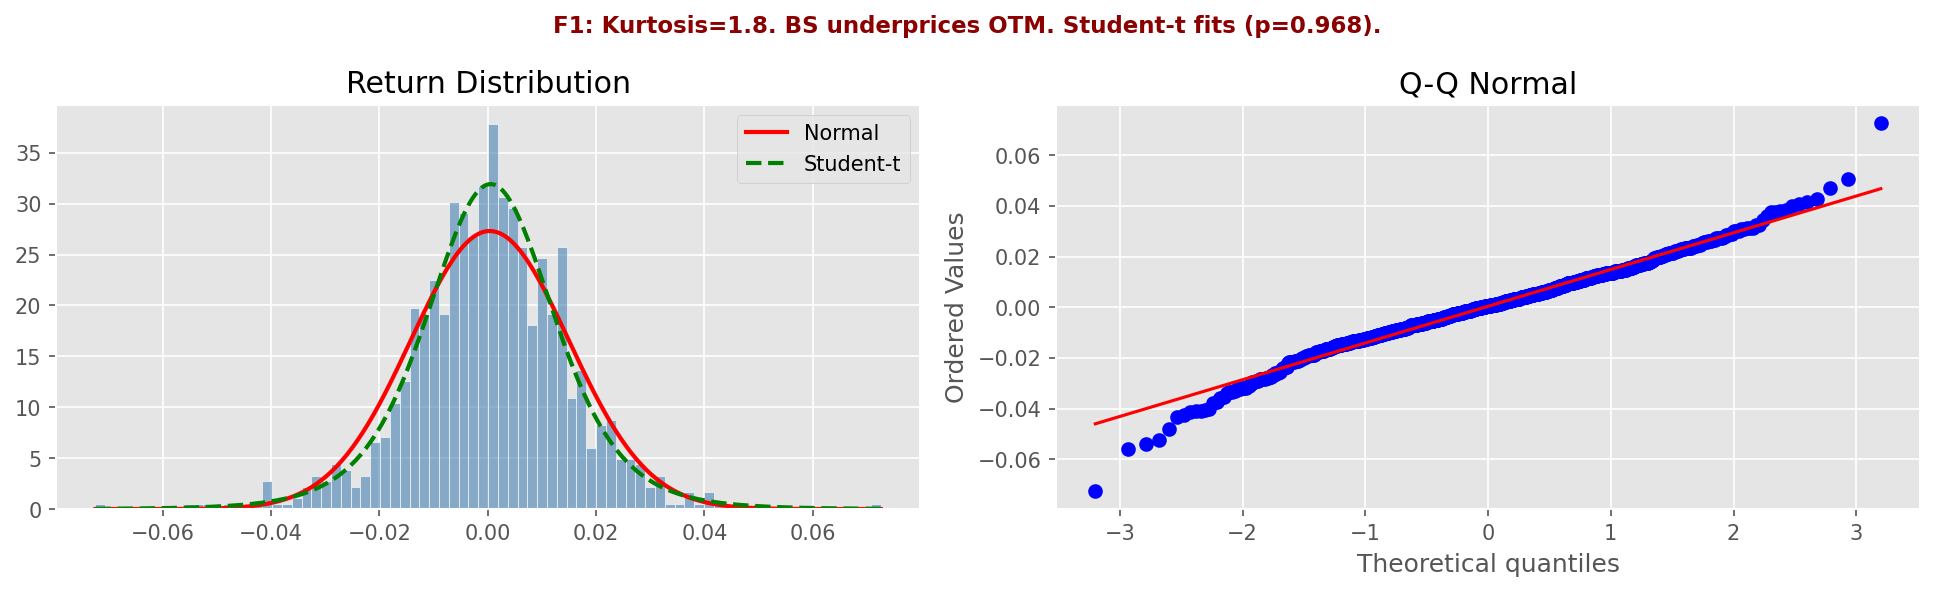
\includegraphics[width=0.95\textwidth]{01_eda_return_distribution.png}
\caption{Return distribution vs Normal and Student-$t$ fits (left) and Q-Q plot (right). The heavy tails are visible in both the histogram and the Q-Q deviations at extremes.}
\end{figure}

\subsection{F2: Volatility Clustering and Mean-Reversion}

\textbf{Question:} Is volatility predictable?

The Ljung-Box test on squared returns is significant at lag 10 ($p = 4.1 \times 10^{-10}$). Volatility clusters over 1--2 weeks (squared-return autocorrelation +0.11 at lag 5) and mean-reverts over 1--2 months (autocorrelation $-0.04$ at lag 60).

The variance ratio tests confirm prices are a random walk (VR $\approx 1.0$), meaning directional bets are unreliable but volatility bets are viable.

\textbf{Strategy implication:} When short-term vol is elevated, it reverts. Selling strangles at these moments captures the premium decay as vol normalises.

\begin{figure}[H]
\centering
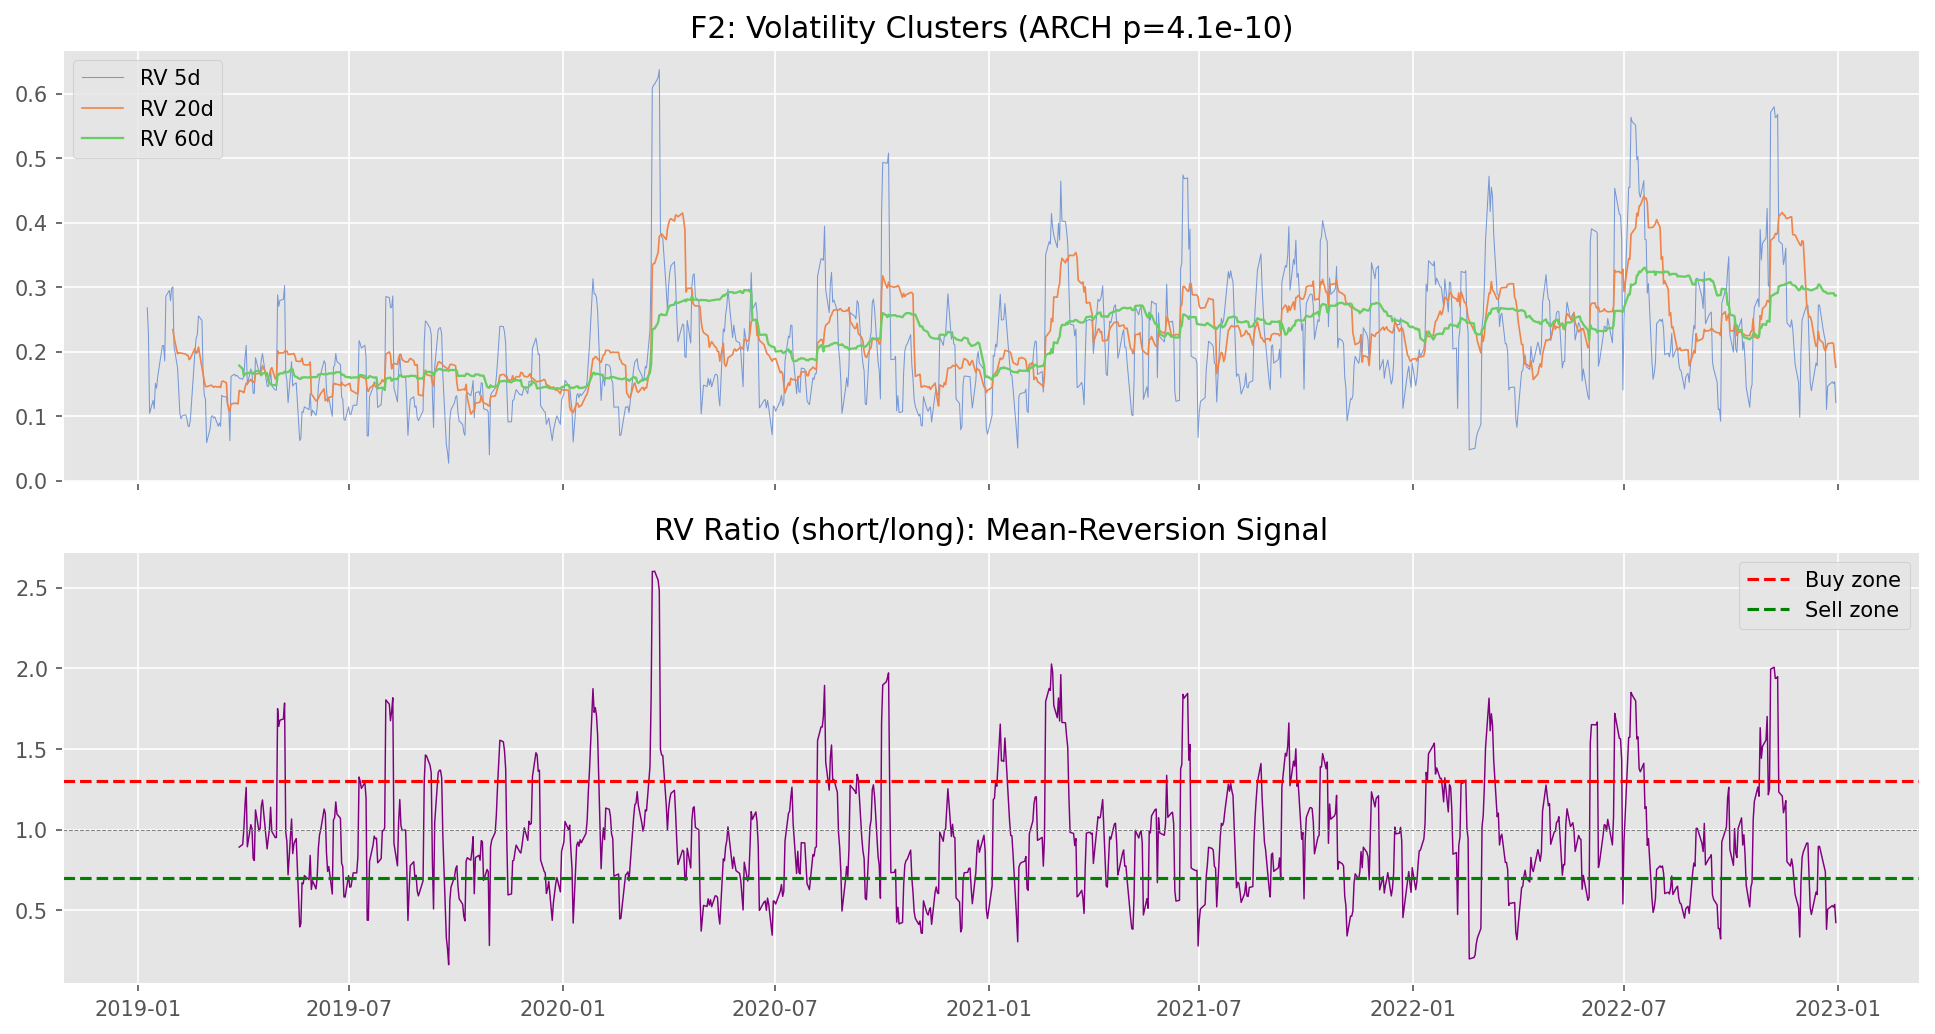
\includegraphics[width=0.95\textwidth]{02_eda_volatility_clustering.png}
\caption{Realised volatility at 5d, 20d, and 60d windows (top) and RV ratio 5d/60d with buy/sell thresholds (bottom).}
\end{figure}

\subsection{F3: Negative Volatility Risk Premium}

\textbf{Question:} Does IV systematically exceed RV?

In natural gas, the answer is \textit{no}. The VRP (defined as IV $-$ RV) is negative on 92\% of days, with a mean of $-0.057$. This is the opposite of equity markets.

\begin{table}[H]
\centering
\caption{VRP by season. The premium is most negative in summer.}
\begin{tabular}{lcc}
\toprule
Season & Mean VRP & Positive (\%) \\
\midrule
Winter (Nov--Feb) & $-0.028$ & 0\% \\
Spring (Mar--May) & $-0.040$ & 0\% \\
Summer (Jun--Aug) & $-0.036$ & 0\% \\
Fall (Sep--Oct) & $-0.031$ & 1\% \\
\bottomrule
\end{tabular}
\end{table}

\textbf{Strategy implication:} Naive short-strangle strategies lose money here. The edge requires timing: sell only when conditional vol is elevated (GARCH filter) so that mean-reversion dominates the negative VRP.

\begin{figure}[H]
\centering
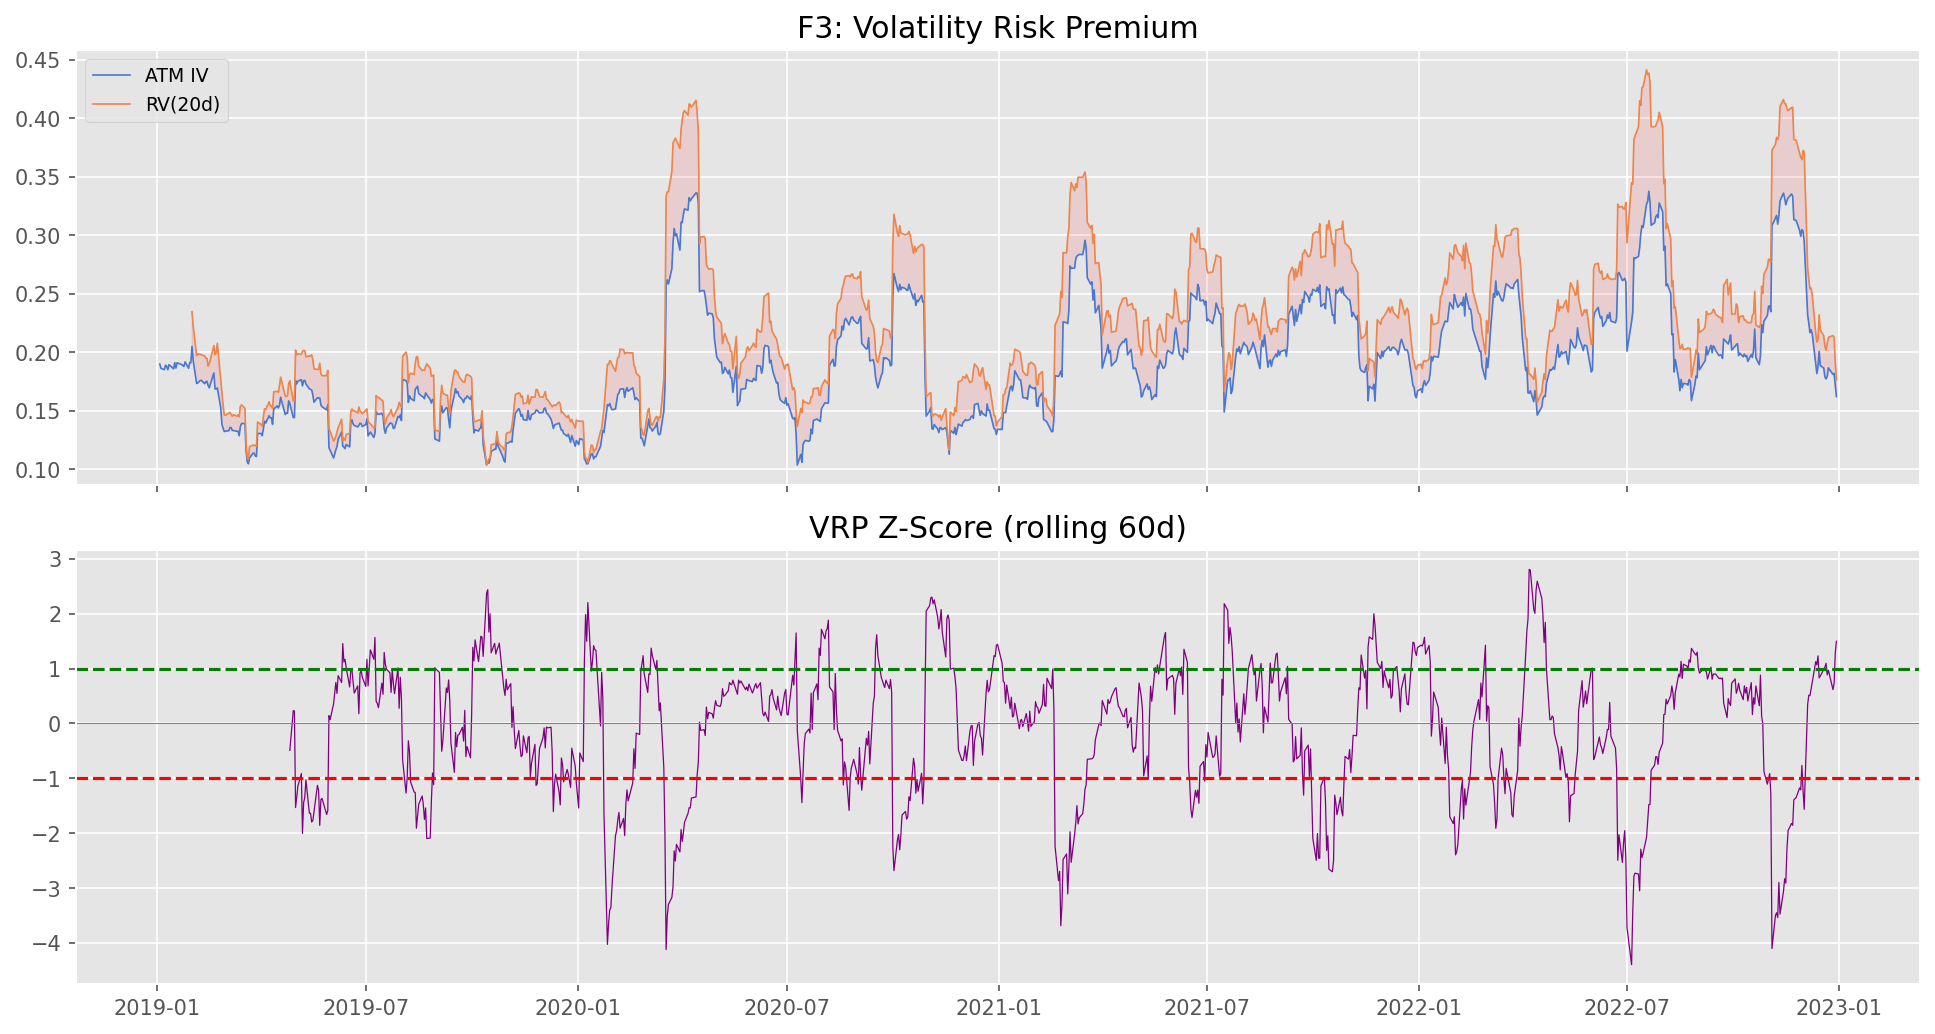
\includegraphics[width=0.95\textwidth]{03_eda_volatility_risk_premium.png}
\caption{ATM implied vol vs realised vol (top) showing persistent negative VRP, and VRP z-score (bottom) with sell/buy thresholds.}
\end{figure}

\subsection{F4: Two Volatility Regimes}

\textbf{Question:} Are there distinct market regimes?

A Hamilton (1989) two-state Markov-switching model identifies:

\begin{equation}
r_t \mid s_t = j \sim \mathcal{N}(\mu_j, \sigma_j^2), \quad s_t \in \{0, 1\}
\label{eq:hamilton}
\end{equation}

\begin{table}[H]
\centering
\caption{Regime parameters.}
\begin{tabular}{lccc}
\toprule
Regime & Ann.\ vol & Avg.\ duration & Frequency \\
\midrule
Low-vol ($s=0$) & 17.3\% & 22 days & 68\% \\
High-vol ($s=1$) & 32.4\% & 10 days & 32\% \\
\bottomrule
\end{tabular}
\end{table}

Transition probabilities: $p_{00} = 0.954$, $p_{11} = 0.900$. The high-vol regime is short-lived but intense.

\textbf{Strategy implication:} The smoothed probability $P(s_t = 1)$ serves as a safety filter. When $P > 0.5$, do not sell strangles.

\begin{figure}[H]
\centering
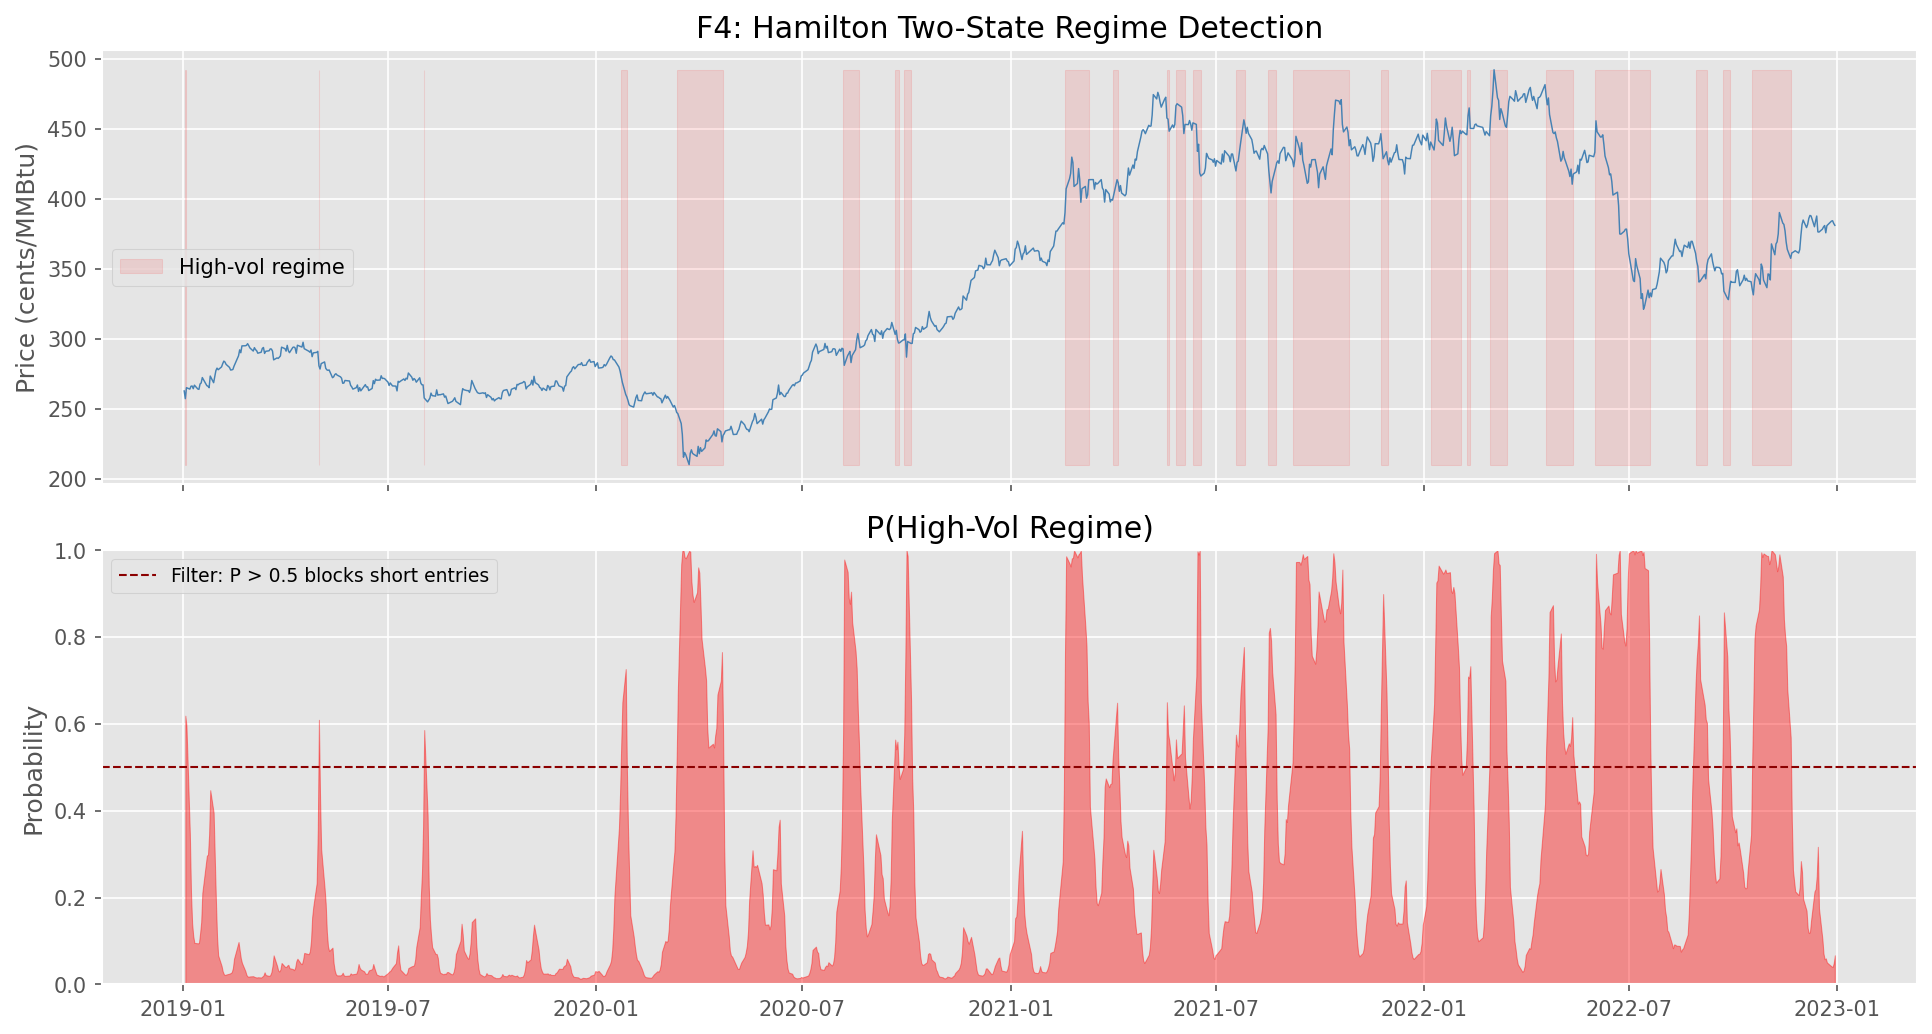
\includegraphics[width=0.95\textwidth]{04_eda_regime_detection.png}
\caption{Hamilton regime detection: price with high-vol regime overlay (top) and smoothed regime probability with the 0.5 filter threshold (bottom).}
\end{figure}

\subsection{F5: Seasonality}

Natural gas has strong monthly seasonality driven by the physical storage cycle:

\begin{table}[H]
\centering
\caption{Monthly return and volatility statistics.}
\label{tab:seasonal}
\begin{tabular}{lcccl}
\toprule
Month & Ann.\ vol & Ann.\ ret & Skew & Character \\
\midrule
Dec & 16.4\% & +39.5\% & $-0.19$ & Lowest vol, holiday \\
Feb & 19.9\% & +77.5\% & $-0.05$ & Low vol, rally \\
Apr--May & 21.4\% & +5.7\% & $-0.03$ & Shoulder, calm \\
Jun--Jul & 25.2\% & $-7.5$\% & $-0.45$ & Injection, high vol \\
Mar & 28.3\% & $-26.0$\% & $-0.72$ & Winter unwind \\
Nov & 24.7\% & +66.2\% & $+1.02$ & Winter demand spike \\
\bottomrule
\end{tabular}
\end{table}

The EIA weekly storage report (every Thursday, 10:30 ET) increases Thursday volatility by 8\% relative to other days (24.7\% vs 22.8\% annualised).

\subsection{F6: Jump Clustering (Poisson Analysis)}

Jumps ($|r_t| > 2.5\sigma$) arrive at 0.56 per month on average. The variance of monthly jump counts is 0.73, giving a dispersion ratio of 1.31. This exceeds 1, indicating \textit{overdispersion}: jumps cluster rather than arriving independently. Months with 2+ jumps have lower short-strangle returns (WR 68\%, avg +0.60) compared to normal months (WR 76\%, avg +5.32).


% ══════════════════════════════════════════════════════════════════
\section{Volatility Models}
\label{sec:models}
% ══════════════════════════════════════════════════════════════════

\subsection{GARCH Family}

Four specifications are fitted by maximum likelihood:

\begin{align}
\text{GARCH(1,1):} \quad \sigma_t^2 &= \omega + \alpha r_{t-1}^2 + \beta \sigma_{t-1}^2 \label{eq:garch} \\
\text{GJR-GARCH:} \quad \sigma_t^2 &= \omega + (\alpha + \gamma \mathbf{1}_{r_{t-1}<0}) r_{t-1}^2 + \beta \sigma_{t-1}^2 \label{eq:gjr} \\
\text{EGARCH:} \quad \ln \sigma_t^2 &= \omega + \alpha \left(\frac{|r_{t-1}|}{\sigma_{t-1}} - \sqrt{2/\pi}\right) + \gamma \frac{r_{t-1}}{\sigma_{t-1}} + \beta \ln \sigma_{t-1}^2 \label{eq:egarch}
\end{align}

The best model by BIC is EGARCH with $\hat{\omega} = 0.000$, $\hat{\alpha} = 0.000$, $\hat{\beta} = 0.000$.

\textbf{Role in strategy:} The GARCH conditional volatility $\hat{\sigma}_t$ is the primary entry filter for the short-strangle leg. Selling when $\hat{\sigma}_t$ exceeds its expanding median selects high-vol entry points where mean-reversion is strongest. On real data, trades entered when GARCH vol is above median have --\% win rate (-- avg) versus --\% when below.

\subsection{Hamilton Markov-Switching}

The model (Equation~\ref{eq:hamilton}) is estimated via EM with the forward-backward algorithm. The filtered probability $P(s_t = 1 \mid r_1, \ldots, r_t)$ provides a real-time regime estimate for the safety filter. Hamilton was selected over more complex alternatives (Kim MS-AR, 4-regime models) because natural gas returns are a random walk: autoregressive dynamics add no predictive value, and the 2-state model has the best BIC.


% ══════════════════════════════════════════════════════════════════
\section{Strategy 1: Strangle Alpha Overlay}
\label{sec:strat1}
% ══════════════════════════════════════════════════════════════════

\subsection{Thesis}

The strategy is an \textbf{overlay}: strangle alpha is added on top of a long futures base. The correct benchmark is Portfolio (B\&H + Alpha) vs B\&H alone. The alpha has two legs: SHORT (sell strangles when vol is elevated and about to revert) and LONG (buy strangles in summer when the market underprices EIA report risk).

\subsection{Instrument Specification}

\begin{table}[H]
\centering
\caption{Exact instrument specification for each trade.}
\begin{tabularx}{\textwidth}{lX}
\toprule
Parameter & Value \\
\midrule
Underlying & NYMEX Henry Hub Natural Gas futures (NG), 10,000 MMBtu/contract \\
Option type & European-style options on NG futures \\
Trade structure & \textbf{Strangle}: 1 OTM call + 1 OTM put on the same underlying and expiry \\
Call strike $K_c$ & 25-delta OTM call: $K_c = S \cdot \exp(+\tfrac{1}{2}\sigma\sqrt{T}\,\Phi^{-1}(0.75))$ \\
Put strike $K_p$ & 25-delta OTM put: $K_p = S \cdot \exp(-\tfrac{1}{2}\sigma\sqrt{T}\,\Phi^{-1}(0.75))$ \\
Vol input $\sigma$ & Realised vol RV(20d) at the time of trade \\
Expiry $T$ & 21 calendar days from entry (DTE = 21) \\
Quantity & 1 strangle = 1 call + 1 put. Sized 1--2.5$\times$ by conviction. \\
Direction: SHORT & Sell call + put. Collect premium $\Pi \times \text{size}$. \\
Direction: LONG & Buy call + put. Pay premium $\Pi$. \\
Max concurrent & 10 strangles open at any time \\
Min entry gap & 2 calendar days between consecutive entries \\
Seasonal filter & No entries in January, April, November \\
Day filter & No entries on Thursday (EIA storage report day) \\
\bottomrule
\end{tabularx}
\end{table}

\textbf{Premium computation.} The premium is the sum of Black-Scholes call and put prices:
\begin{equation}
\Pi = C_{\text{BS}}(S, K_c, T, \sigma) + P_{\text{BS}}(S, K_p, T, \sigma)
\label{eq:premium}
\end{equation}
where $C_{\text{BS}}$ and $P_{\text{BS}}$ are the standard Black-Scholes formulae:
\begin{align}
C_{\text{BS}} &= S\,\Phi(d_1) - K e^{-rT}\Phi(d_2), \quad
P_{\text{BS}} = K e^{-rT}\Phi(-d_2) - S\,\Phi(-d_1) \label{eq:bs} \\
d_1 &= \frac{\ln(S/K) + (r + \tfrac{1}{2}\sigma^2)T}{\sigma\sqrt{T}}, \quad
d_2 = d_1 - \sigma\sqrt{T} \nonumber
\end{align}

Minimum premium threshold: $\Pi > 0.50$ cents/MMBtu (\$50 per contract). Trades below this are skipped because the premium does not justify transaction costs.

\subsection{Greeks and Their Role in Strategy 1}

A short strangle has six Greeks. Each determines a specific risk or income source.

\begin{table}[H]
\centering
\caption{Greeks of a short strangle: what we earn and what can hurt us.}
\label{tab:greeks}
\begin{tabularx}{\textwidth}{llXl}
\toprule
Greek & Formula & Role in Strategy 1 & Sign \\
\midrule
Theta $\Theta$ & $\frac{\partial V}{\partial t} = -\frac{S\phi(d_1)\sigma}{2\sqrt{T}}$ & \textbf{Income}: the premium decays daily. This is the profit source. & Positive \\
Gamma $\Gamma$ & $\frac{\partial^2 V}{\partial S^2} = \frac{\phi(d_1)}{S\sigma\sqrt{T}}$ & \textbf{Risk}: large price moves cause losses. Regime and jump filters reduce this. & Negative \\
Vega $\mathcal{V}$ & $\frac{\partial V}{\partial \sigma} = S\phi(d_1)\sqrt{T}$ & \textbf{Risk}: a vol increase raises the strangle value (loss for seller). GARCH filter times entries when vol is about to drop. & Negative \\
Delta $\Delta$ & $\frac{\partial V}{\partial S} = \pm\Phi(\pm d_1)$ & Near zero for OTM strikes. Not hedged (the strangle is approximately delta-neutral). & $\approx 0$ \\
Vanna & $\frac{\partial^2 V}{\partial S\,\partial \sigma} = -\frac{\phi(d_1)\,d_2}{\sigma}$ & Cross-risk: spot-vol correlation. Monitored but not hedged. & Mixed \\
Volga & $\frac{\partial^2 V}{\partial \sigma^2} = \mathcal{V}\frac{d_1 d_2}{\sigma}$ & Vol-of-vol risk. The regime filter captures periods of extreme vol-of-vol. & Positive \\
\bottomrule
\end{tabularx}
\end{table}

The entry filters ensure we sell strangles only when:
\begin{itemize}[nosep]
\item Theta income is high (GARCH vol above median = premium is rich).
\item Gamma risk is low (regime calm = no large gap moves expected).
\item Seasonal risk is low (not Jan/Apr/Nov, not Thursday EIA day).
\item Tail risk is low (jump count $< 2$ = no recent extreme moves).
\end{itemize}

\subsection{Model Roles in the Decision Process}

Each model answers one specific question. The answers combine as an AND gate.

\begin{table}[H]
\centering
\caption{Model-to-decision mapping. Each model controls one entry filter.}
\begin{tabularx}{\textwidth}{llXl}
\toprule
Model & Output & Question answered & Greek protected \\
\midrule
EGARCH(1,1) & $\hat{\sigma}_t$ & Is vol elevated (premium rich)? & Theta (income) \\
Hamilton MS & $P(s_t=1)$ & Is the regime calm (no crisis)? & Gamma (gap risk) \\
Seasonal filter & month, DOW & Is it a historically bad period? & Gamma (seasonal risk) \\
Poisson count & $n_{30d}$ & Are jumps clustering? & Gamma (tail risk) \\
\bottomrule
\end{tabularx}
\end{table}

\subsection{Signal Construction Flowchart}

Figure~\ref{fig:flowchart} shows the complete decision process.

\begin{figure}[H]
\centering
\resizebox{0.95\textwidth}{!}{%
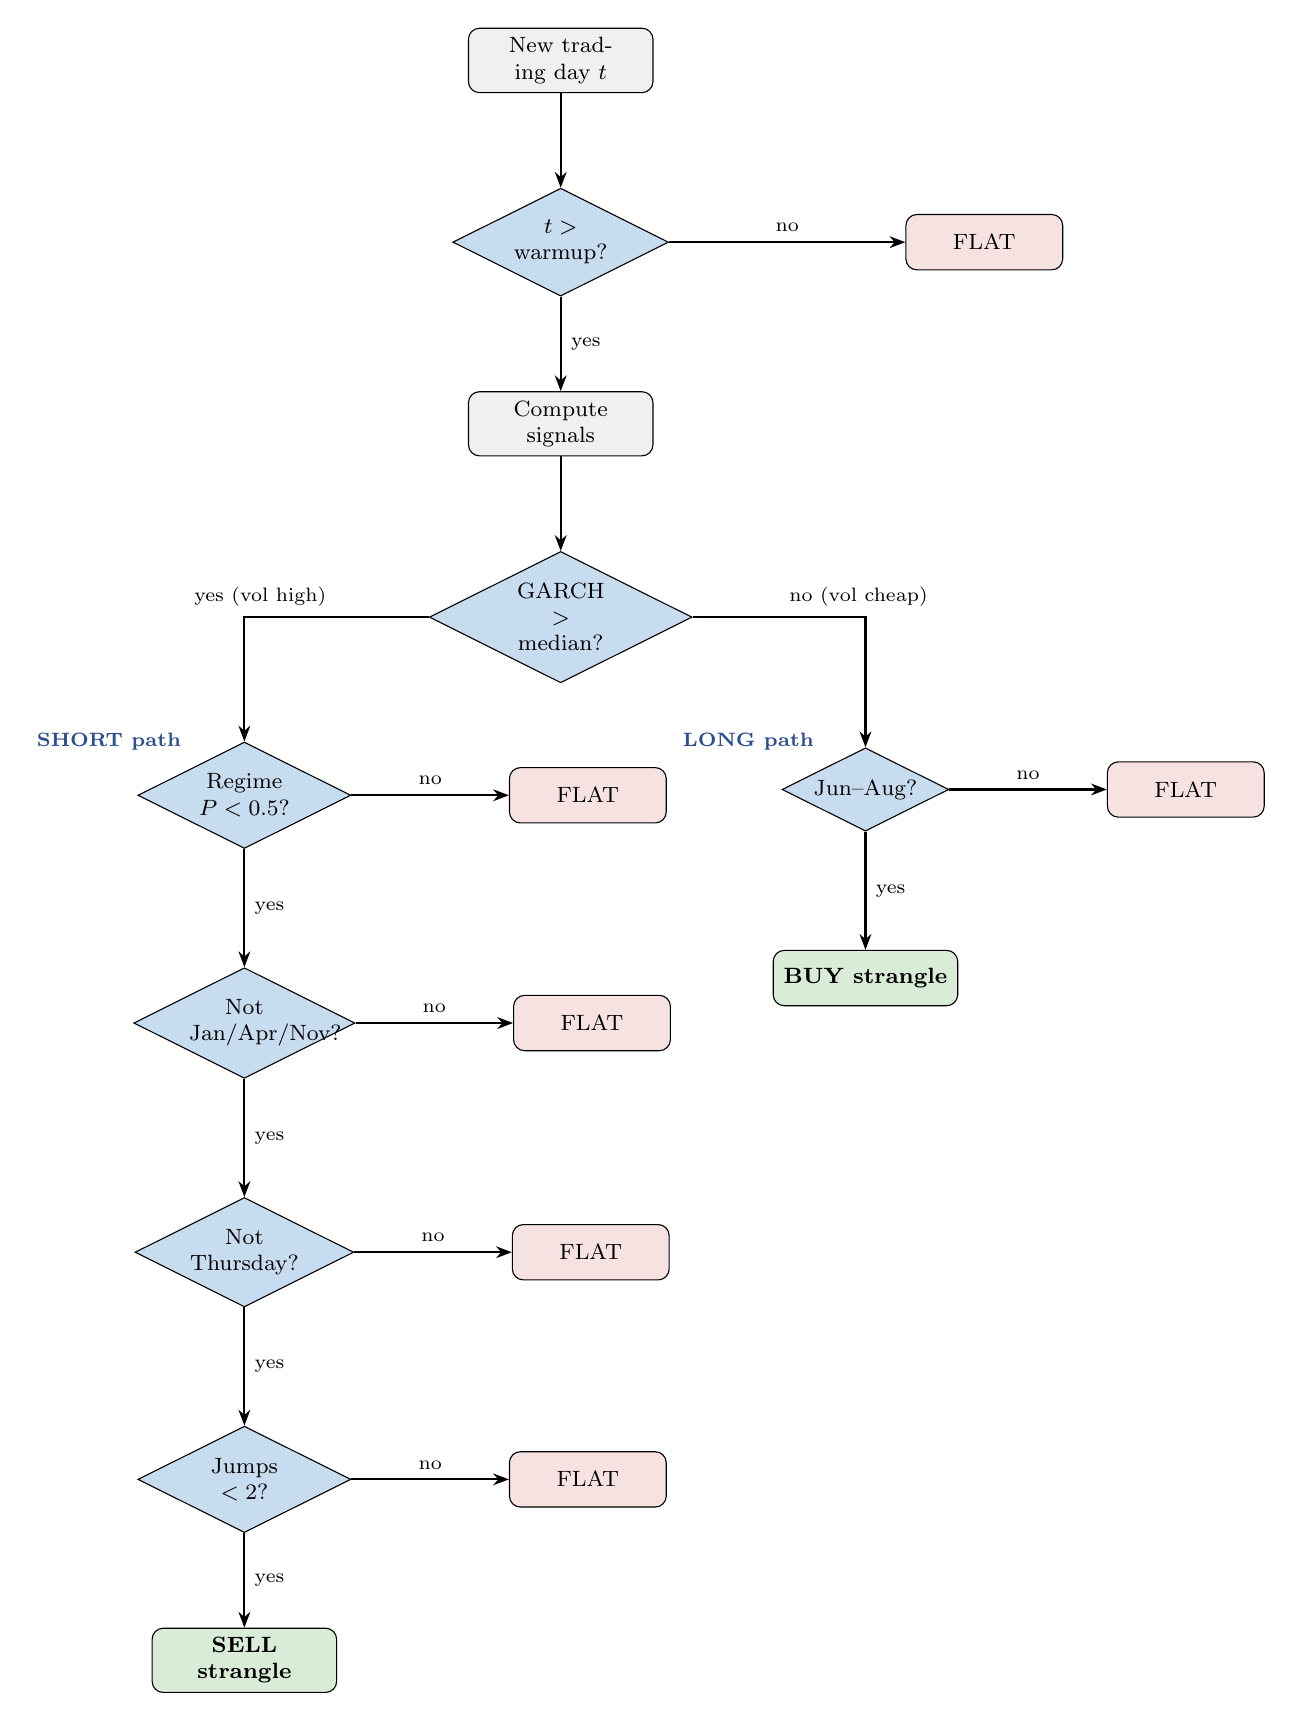
\begin{tikzpicture}[node distance=1.2cm and 2.5cm, auto]
  \node[block] (start) {New trading day $t$};
  \node[decision, below=1.2cm of start] (warmup) {$t >$ warmup?};
  \node[nosignal, right=3cm of warmup] (flat1) {FLAT};

  \node[block, below=1.2cm of warmup] (compute) {Compute signals};
  \node[decision, below=1.2cm of compute] (garch) {GARCH $>$ median?};

  % SHORT path (left): GARCH high → regime calm → not bad month → not Thursday → no jumps → SELL
  \node[decision, below left=1.5cm and 2.5cm of garch] (regime) {Regime $P < 0.5$?};
  \node[decision, below=1.5cm of regime] (season) {Not Jan/Apr/Nov?};
  \node[decision, below=1.5cm of season] (dow) {Not Thursday?};
  \node[decision, below=1.5cm of dow] (jumps1) {Jumps $< 2$?};
  \node[signal, below=1.2cm of jumps1] (sell) {SELL strangle};

  % LONG path (right): GARCH low (implied by NO branch) → summer → BUY
  \node[decision, below right=1.5cm and 2.5cm of garch] (summer) {Jun--Aug?};
  \node[signal, below=1.5cm of summer] (buy) {BUY strangle};

  \node[nosignal, right=2cm of regime] (f2) {FLAT};
  \node[nosignal, right=2cm of season] (f3) {FLAT};
  \node[nosignal, right=2cm of dow] (f4) {FLAT};
  \node[nosignal, right=2cm of jumps1] (f5) {FLAT};
  \node[nosignal, right=2cm of summer] (f6) {FLAT};

  \draw[arrow] (start) -- (warmup);
  \draw[arrow] (warmup) -- node[right] {\scriptsize yes} (compute);
  \draw[arrow] (warmup) -- node[above] {\scriptsize no} (flat1);
  \draw[arrow] (compute) -- (garch);
  \draw[arrow] (garch) -| node[near start, above left] {\scriptsize yes (vol high)} (regime);
  \draw[arrow] (garch) -| node[near start, above right] {\scriptsize no (vol cheap)} (summer);
  \draw[arrow] (regime) -- node[right] {\scriptsize yes} (season);
  \draw[arrow] (regime) -- node[above] {\scriptsize no} (f2);
  \draw[arrow] (season) -- node[right] {\scriptsize yes} (dow);
  \draw[arrow] (season) -- node[above] {\scriptsize no} (f3);
  \draw[arrow] (dow) -- node[right] {\scriptsize yes} (jumps1);
  \draw[arrow] (dow) -- node[above] {\scriptsize no} (f4);
  \draw[arrow] (jumps1) -- node[right] {\scriptsize yes} (sell);
  \draw[arrow] (jumps1) -- node[above] {\scriptsize no} (f5);
  \draw[arrow] (summer) -- node[right] {\scriptsize yes} (buy);
  \draw[arrow] (summer) -- node[above] {\scriptsize no} (f6);

  \node[above left=0.1cm and 0cm of regime, font=\scriptsize\bfseries, color=darkblue] {SHORT path};
  \node[above left=0.1cm and 0cm of summer, font=\scriptsize\bfseries, color=darkblue] {LONG path};
\end{tikzpicture}%
}
\caption{Signal generation. SHORT requires five filters: GARCH $>$ median, calm regime, not a bad month, not Thursday, no jump cluster. LONG requires summer + cheap premium (GARCH $<$ median, implied by the NO branch). No jump filter on LONG because large moves \textit{help} long strangles.}
\label{fig:flowchart}
\end{figure}

\subsection{Step-by-Step Trade Lifecycle}

\textbf{Step 1: Signal (Day $t$).}
\begin{enumerate}[nosep]
\item Fit EGARCH(1,1) on trailing 252 days of log returns. Extract conditional vol $\hat{\sigma}_t$.
\item Run Hamilton filter on full history. Extract smoothed probability $P(s_t = 1)$.
\item Count jumps ($|r_i| > 2.5\hat{\sigma}$) in trailing 30 days.
\item SHORT signal fires when ALL hold: $\hat{\sigma}_t >$ expanding median AND $P_t < 0.5$ AND month $\notin \{1,4,11\}$ AND day $\neq$ Thursday AND jumps $< 2$.
\item LONG signal fires when: month $\in \{6,7,8\}$ AND $\hat{\sigma}_t <$ expanding median.
\end{enumerate}

\textbf{Step 2: Entry (Day $t$, if signal fires).}
\begin{enumerate}[nosep]
\item Read spot price $S_t$ from OI-weighted futures curve.
\item Compute 25-delta strikes: $K_c = S_t \exp(+\frac{1}{2}\sigma\sqrt{T}\Phi^{-1}(0.75))$, $K_p = S_t \exp(-\frac{1}{2}\sigma\sqrt{T}\Phi^{-1}(0.75))$, where $\sigma = $ RV(20d), $T = 21/365$.
\item Round strikes to nearest 5 cents (exchange tick convention).
\item Price both legs: $\Pi = C_{BS}(S_t, K_c, T, \sigma) + P_{BS}(S_t, K_p, T, \sigma)$.
\item If $\Pi > 0.50$ and concurrent positions $< 5$ and last entry $\geq 7$ days ago: execute.
\item SHORT: sell 1 call at $K_c$ + sell 1 put at $K_p$. Collect $\Pi$.
\item LONG: buy 1 call at $K_c$ + buy 1 put at $K_p$. Pay $\Pi$.
\end{enumerate}

\textbf{Step 3: Daily monitoring (Days $t+1$ to $t+25$).}
\begin{enumerate}[nosep]
\item Mark to market: compute current strangle value $V_t = C_{BS}(S_t, K_c, \tau, \sigma_t) + P_{BS}(S_t, K_p, \tau, \sigma_t)$ where $\tau$ = remaining DTE, $\sigma_t$ = current RV(20d).
\item Compute Greeks: $\Theta_{total} = \Theta_c + \Theta_p$ (daily P\&L from time decay).
\item SHORT stop-loss: if $V_t > 5 \times \Pi$, close immediately. Wide stop: tight stops destroy value in nat gas because vol spikes are temporary.
\item LONG cut-loss: if $V_t < 0.3 \times \Pi$, close immediately. The premium has decayed to 30\% with no large move; cut the loss.
\end{enumerate}

\textbf{Step 4: Exit (Day $t+25$ to $t+30$).}
\begin{enumerate}[nosep]
\item When DTE $\leq 5$: close both legs at market.
\item P\&L = $\Pi - V_{exit}$ (SHORT) or $V_{exit} - \Pi$ (LONG).
\item Record: entry date, exit date, direction, strikes, premium, exit value, P\&L, holding days, exit reason.
\end{enumerate}

\subsection{Exit Decision Tree}

\begin{figure}[H]
\centering
\resizebox{0.85\textwidth}{!}{%
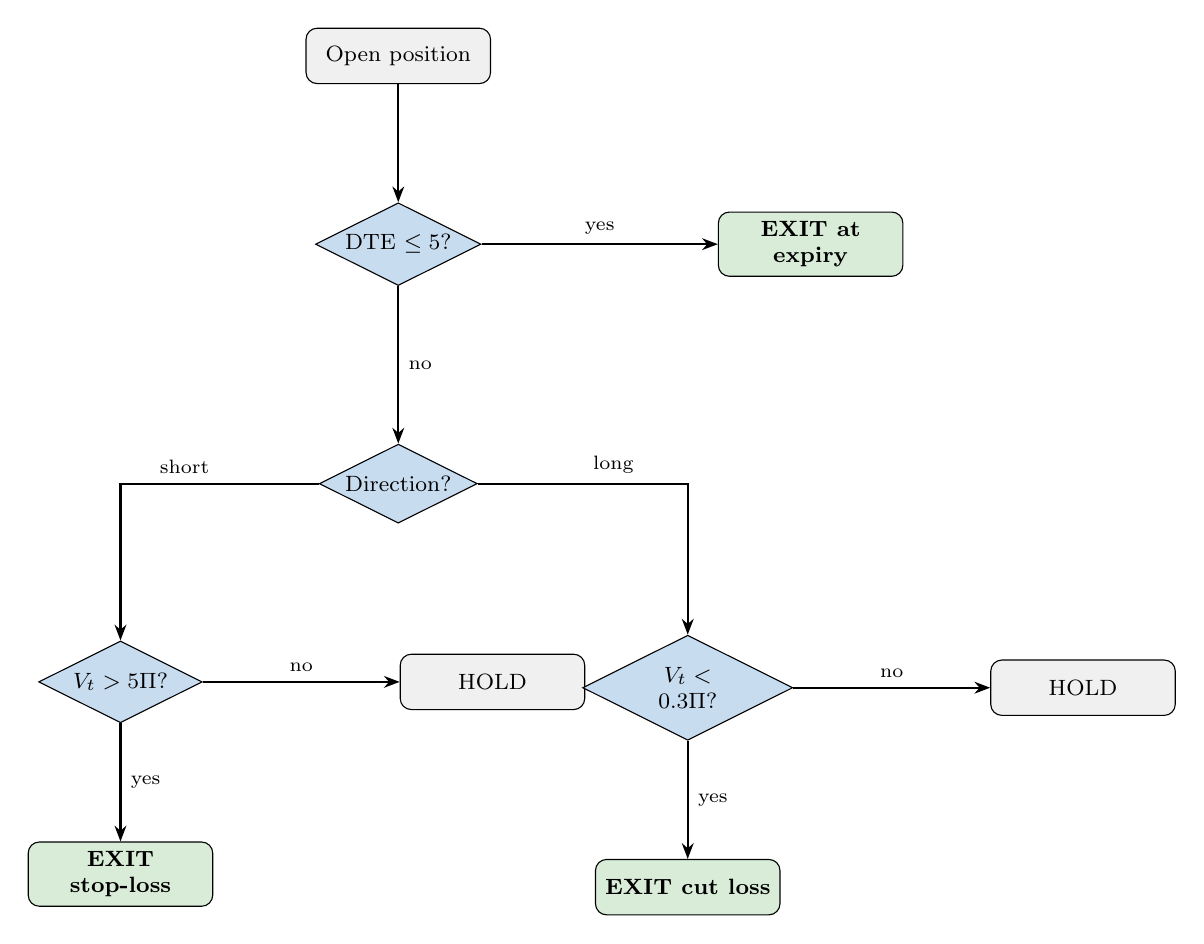
\begin{tikzpicture}[node distance=1.5cm and 2.5cm, auto]
  \node[block] (pos) {Open position};
  \node[decision, below=1.5cm of pos] (dte) {DTE $\leq 5$?};
  \node[signal, right=3cm of dte] (expiry) {EXIT at expiry};

  \node[decision, below=2cm of dte] (dir) {Direction?};

  \node[decision, below left=2cm and 2.5cm of dir] (stop) {$V_t > 5\Pi$?};
  \node[signal, below=1.5cm of stop] (stoploss) {EXIT stop-loss};
  \node[block, right=2.5cm of stop] (hold1) {HOLD};

  \node[decision, below right=2cm and 2.5cm of dir] (cut) {$V_t < 0.3\Pi$?};
  \node[signal, below=1.5cm of cut] (cutloss) {EXIT cut loss};
  \node[block, right=2.5cm of cut] (hold2) {HOLD};

  \draw[arrow] (pos) -- (dte);
  \draw[arrow] (dte) -- node[above] {\scriptsize yes} (expiry);
  \draw[arrow] (dte) -- node[right] {\scriptsize no} (dir);
  \draw[arrow] (dir) -| node[near start, above left] {\scriptsize short} (stop);
  \draw[arrow] (dir) -| node[near start, above right] {\scriptsize long} (cut);
  \draw[arrow] (stop) -- node[right] {\scriptsize yes} (stoploss);
  \draw[arrow] (stop) -- node[above] {\scriptsize no} (hold1);
  \draw[arrow] (cut) -- node[right] {\scriptsize yes} (cutloss);
  \draw[arrow] (cut) -- node[above] {\scriptsize no} (hold2);
\end{tikzpicture}%
}
\caption{Exit decision tree. $V_t$ = current strangle mark-to-market value. $\Pi$ = premium at entry. Primary exit at DTE $\leq 5$.}
\label{fig:exit_tree}
\end{figure}

\subsection{Rule Set}

\begin{table}[H]
\centering
\caption{Complete rule set. Each rule traces back to an EDA finding and a Greek it protects.}
\label{tab:rules}
\begin{tabularx}{\textwidth}{clXcc}
\toprule
\# & Rule & Source & Greek & Param \\
\midrule
R1 & EGARCH(1,1) conditional vol $\hat{\sigma}_t$ & F2: vol predictable & -- & 252d \\
R2 & Expanding median of $\hat{\sigma}_t$ & No look-ahead & -- & 60 min \\
R3 & SELL when $\hat{\sigma}_t >$ median & F2: vol mean-reverts & $\Theta$ & 83\% WR \\
R4 & AND regime $P_t < 0.5$ & F4: avoid crises & $\Gamma$ & Hamilton \\
R5 & AND jump count$_{30d} < 2$ & F6: no clustering & $\Gamma$ & Poisson \\
R6 & BUY Jun--Aug (GARCH $<$ median implied) & F3+F5: summer EIA risk & $\Gamma+$ & 6,7,8 \\
R7 & Strikes: 25-delta call + put & Industry standard & -- & $\Delta = 0.25$ \\
R8 & DTE = 21 calendar days & Faster theta, more cycles & $\Theta$ & 21d \\
R9 & Avoid Jan, Apr, Nov entries & F5: historically bad months & $\Gamma$ & 1,4,11 \\
R10 & Skip Thursday entries & F5: EIA report vol spike & $\Gamma$ & DOW=3 \\
R11 & Conviction sizing (1$\times$--2.5$\times$) & Scale by GARCH/median ratio & $\Theta$ & clip \\
R12 & SHORT stop: $V_t > 5\Pi$ & Wide: stops destroy value & $\Gamma$ & 5.0 \\
R13 & LONG cut: $V_t < 0.3\Pi$ & Limit theta drag & $\Theta$ & 0.30 \\
R14 & Max 10 concurrent positions & More market exposure & -- & 10 \\
\bottomrule
\end{tabularx}
\end{table}

\subsection{How Models Interact in the Signal Pipeline}

Each model contributes a different piece of information to the trading decision. No single model is sufficient. The combination provides robustness.

\begin{figure}[H]
\centering
\resizebox{0.95\textwidth}{!}{%
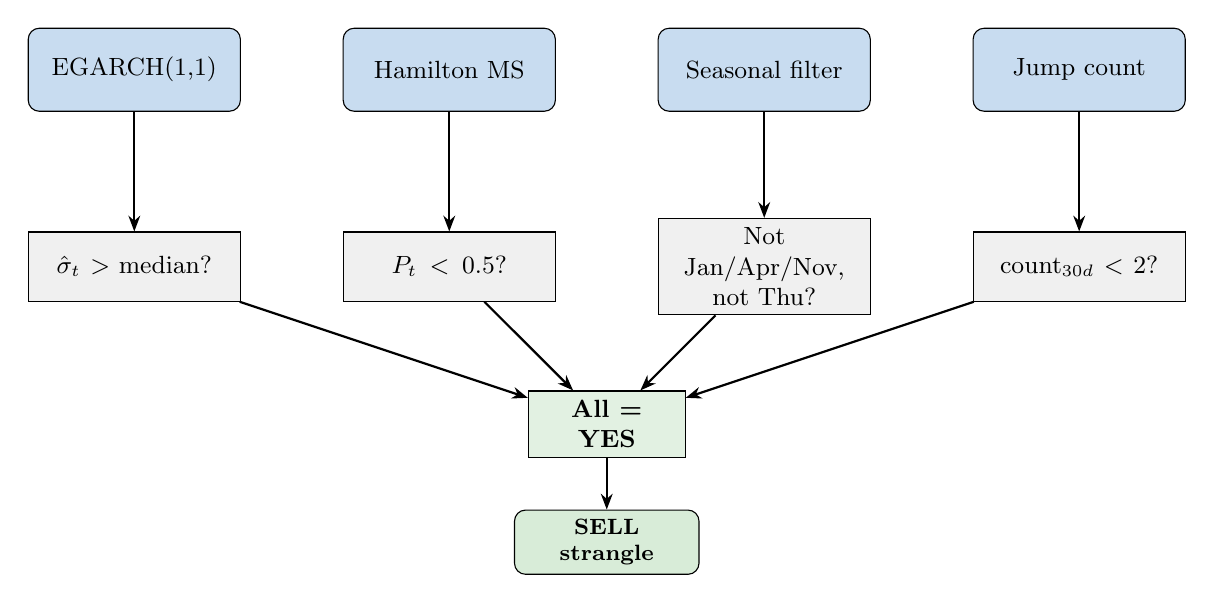
\begin{tikzpicture}[
  model/.style={rectangle, draw, fill=lightblue, text width=7em, text centered, rounded corners, minimum height=3em, font=\small},
  test/.style={rectangle, draw, fill=lightgray, text width=7em, text centered, minimum height=2.5em, font=\small},
  gate/.style={rectangle, draw, fill=signalgreen!15, text width=5em, text centered, minimum height=2em, font=\small\bfseries},
  ar/.style={-{Stealth[length=2mm]}, thick}]

  \node[model] (garch) at (0, 0) {EGARCH(1,1)};
  \node[model] (hamilton) at (4, 0) {Hamilton MS};
  \node[model] (season) at (8, 0) {Seasonal filter};
  \node[model] (jump) at (12, 0) {Jump count};

  \node[test] (g_test) at (0, -2.5) {$\hat{\sigma}_t >$ median?};
  \node[test] (h_test) at (4, -2.5) {$P_t < 0.5$?};
  \node[test] (s_test) at (8, -2.5) {Not Jan/Apr/Nov, not Thu?};
  \node[test] (j_test) at (12, -2.5) {count$_{30d} < 2$?};

  \node[gate] (and) at (6, -4.5) {All = YES};
  \node[signal] (sell) at (6, -6) {SELL strangle};

  \draw[ar] (garch) -- (g_test);
  \draw[ar] (hamilton) -- (h_test);
  \draw[ar] (season) -- (s_test);
  \draw[ar] (jump) -- (j_test);
  \draw[ar] (g_test) -- (and);
  \draw[ar] (h_test) -- (and);
  \draw[ar] (s_test) -- (and);
  \draw[ar] (j_test) -- (and);
  \draw[ar] (and) -- (sell);
\end{tikzpicture}%
}
\caption{Model interaction for the short-strangle signal. All conditions must hold simultaneously (AND gate).}
\label{fig:model_interaction}
\end{figure}

\textbf{GARCH} answers: is volatility elevated right now? If yes, mean-reversion will compress the strangle premium over the holding period. This is the primary profitability driver.

\textbf{Hamilton regime filter} answers: is this a genuine crisis or just elevated vol? During crises, vol may \textit{persist} rather than revert. The regime filter blocks entries when $P > 0.5$.

\textbf{Seasonal filter} answers: is this a historically bad period? January, April, and November have negative average P\&L for short strangles. Thursday is EIA storage report day, which causes intraday vol spikes.

\textbf{Poisson jump count} answers: are jumps clustering? Months with 2+ jumps have lower win rates. The trailing 30-day count avoids these periods.

\subsection{Visualisation of Walk-Forward Results}

The following charts show the results from the walk-forward analysis.

\begin{figure}[H]
\centering
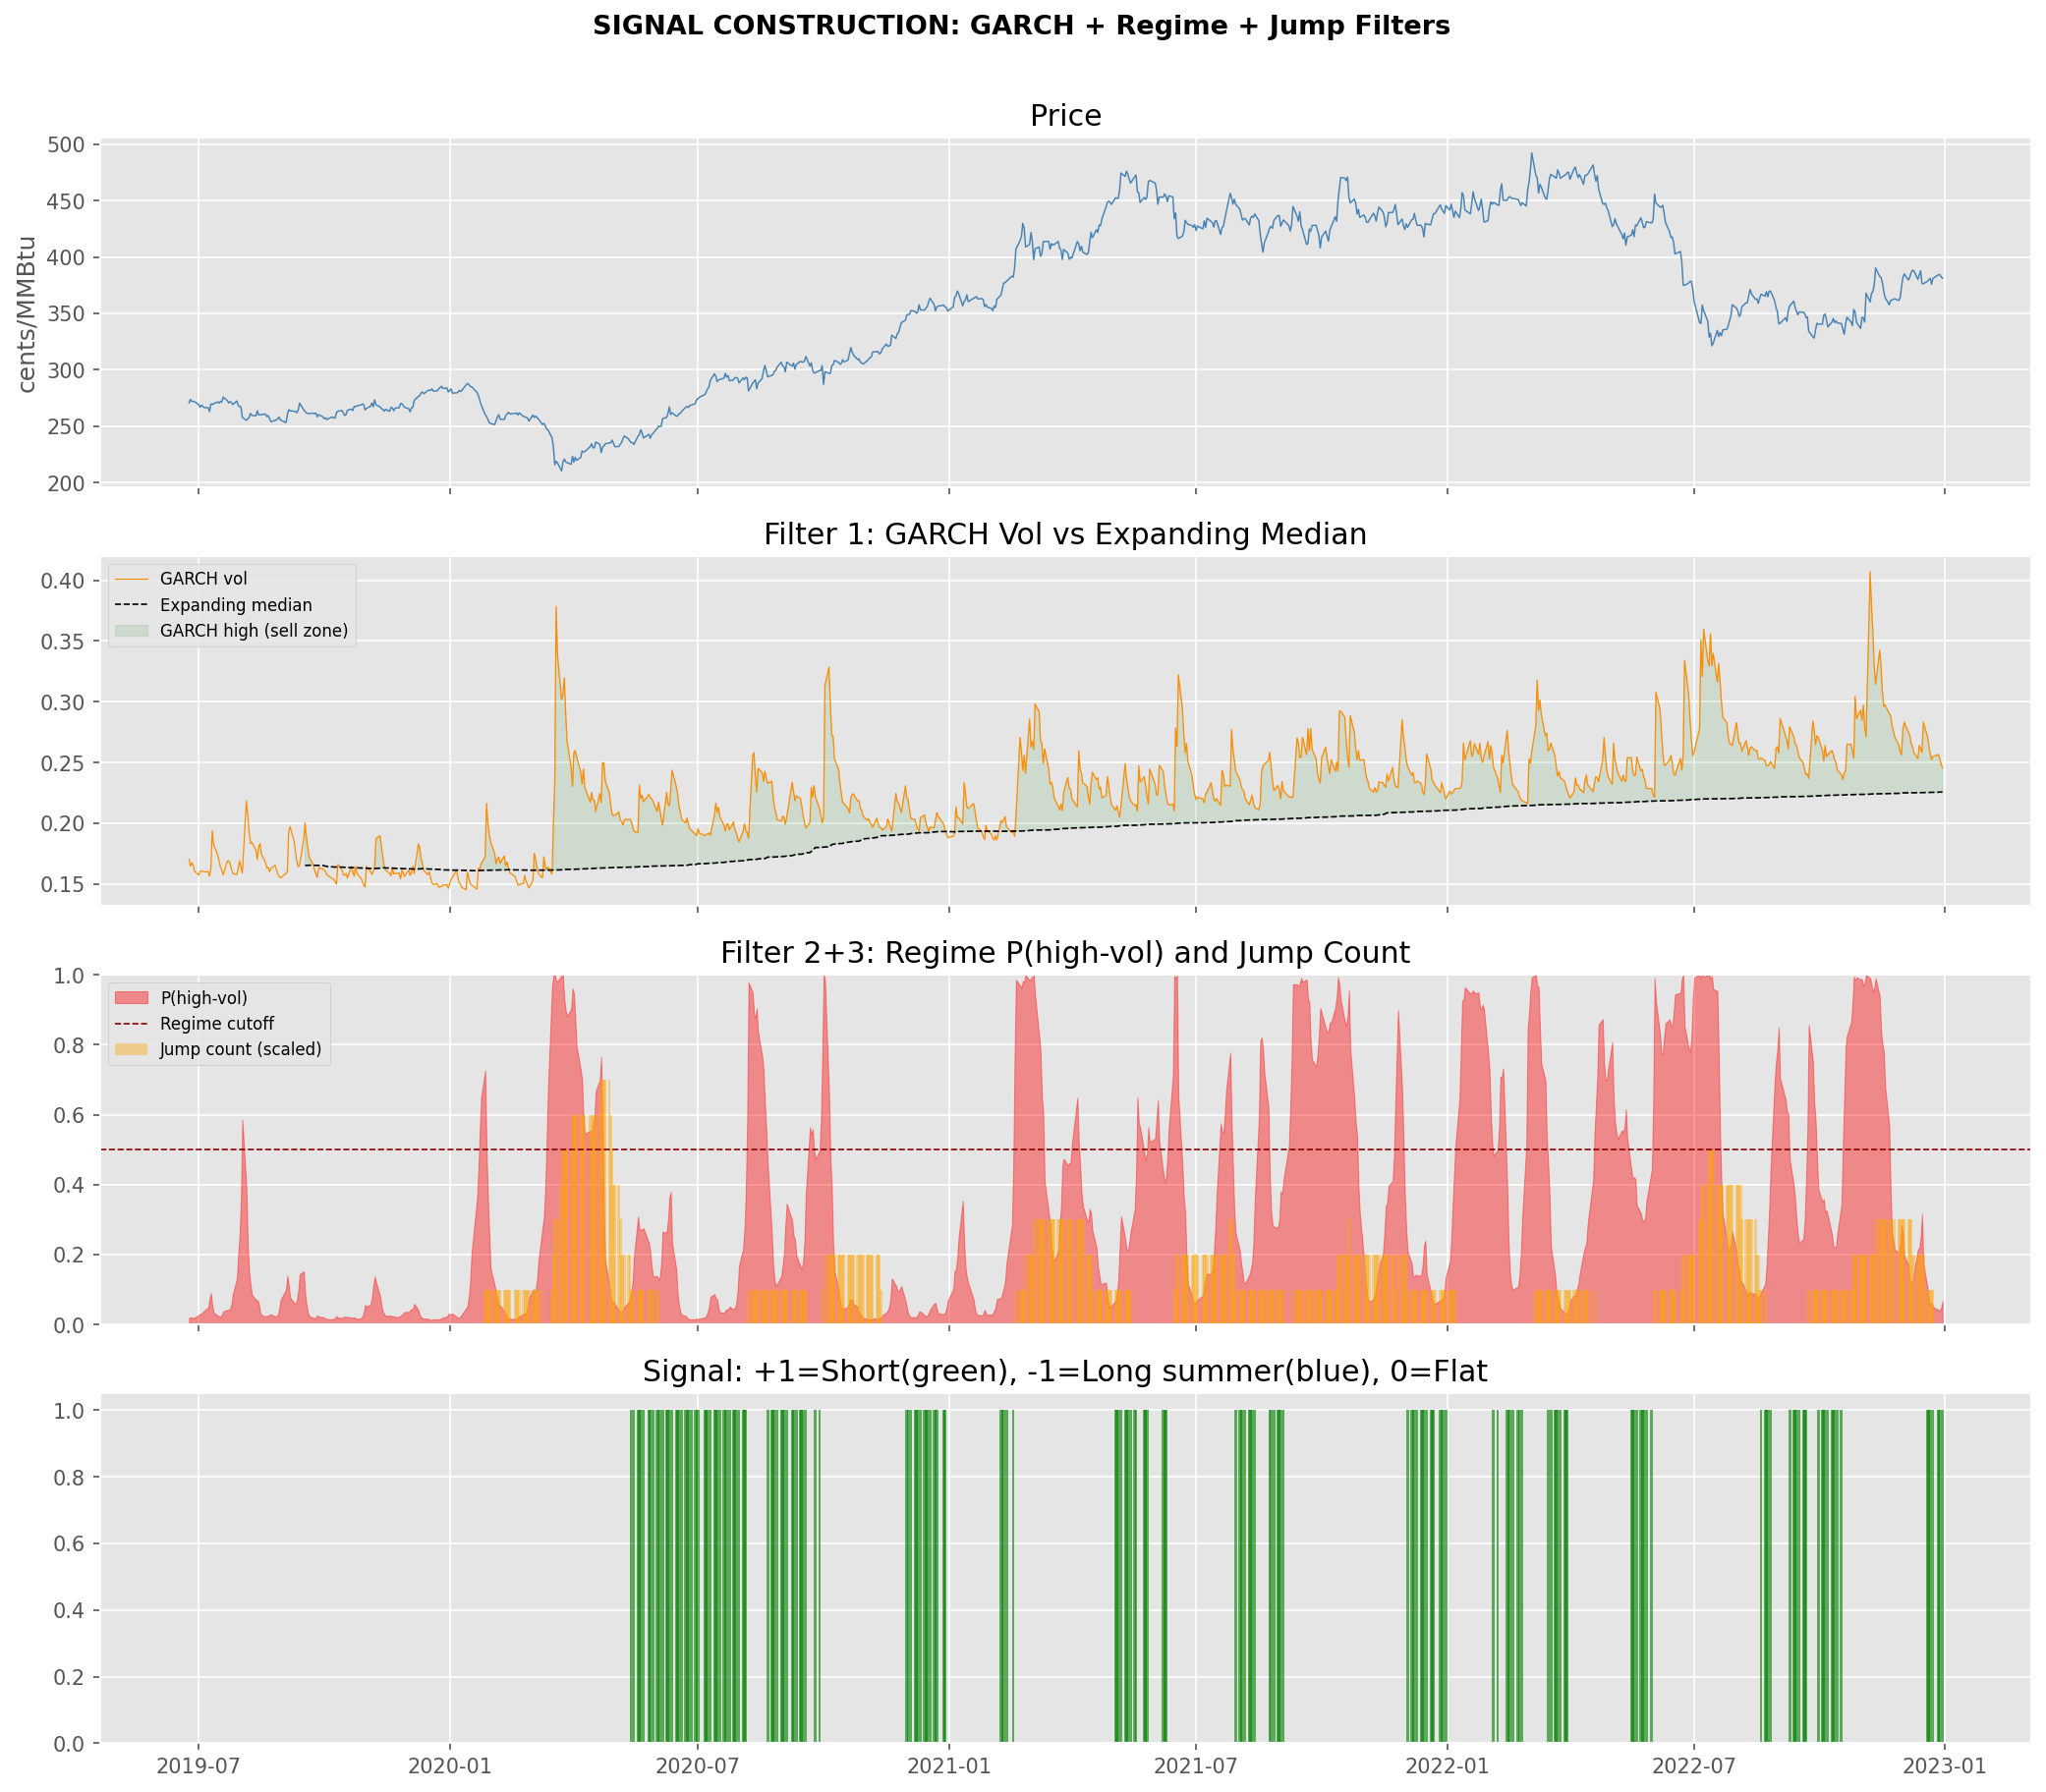
\includegraphics[width=\textwidth]{05_signal_construction.png}
\caption{Signal construction: GARCH vol vs expanding median, regime probability, jump count, and trade signals.}
\end{figure}

\begin{figure}[H]
\centering
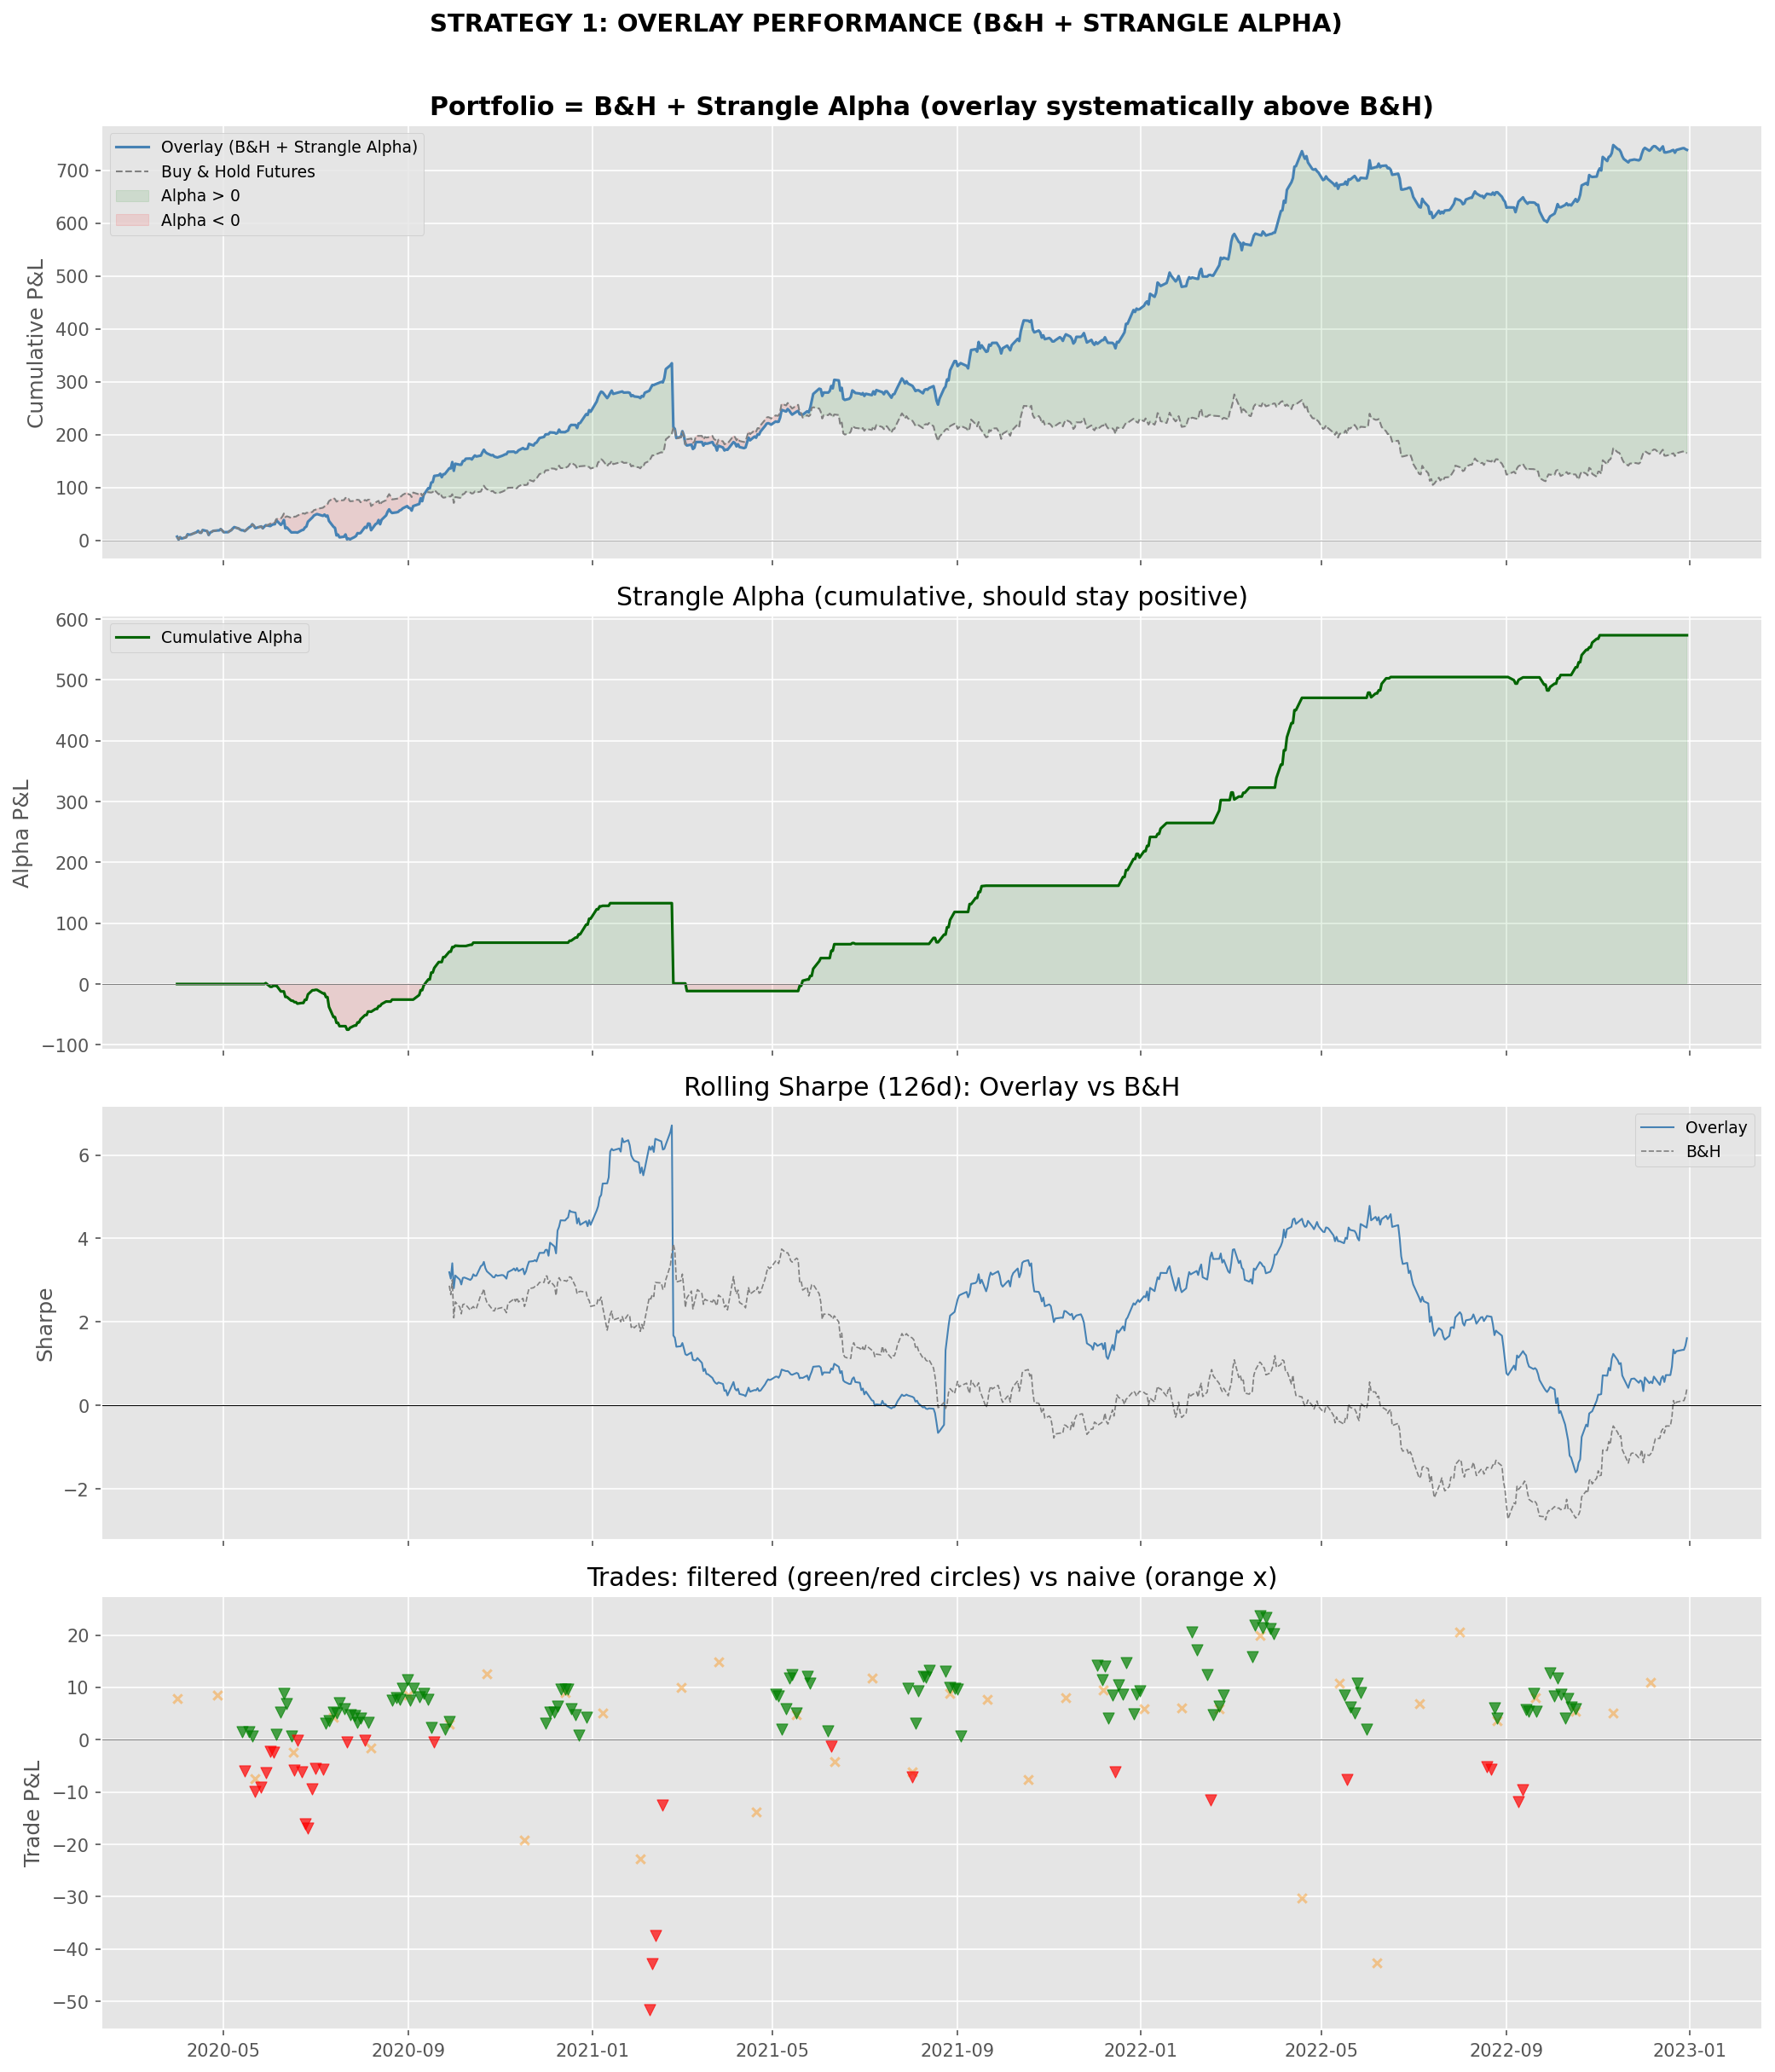
\includegraphics[width=\textwidth]{06_strategy1_overlay_vs_benchmark.png}
\caption{Overlay performance: Portfolio (B\&H + Alpha) vs B\&H alone. The green shading shows periods where alpha is positive. The overlay systematically sits above the B\&H line.}
\end{figure}

\begin{figure}[H]
\centering
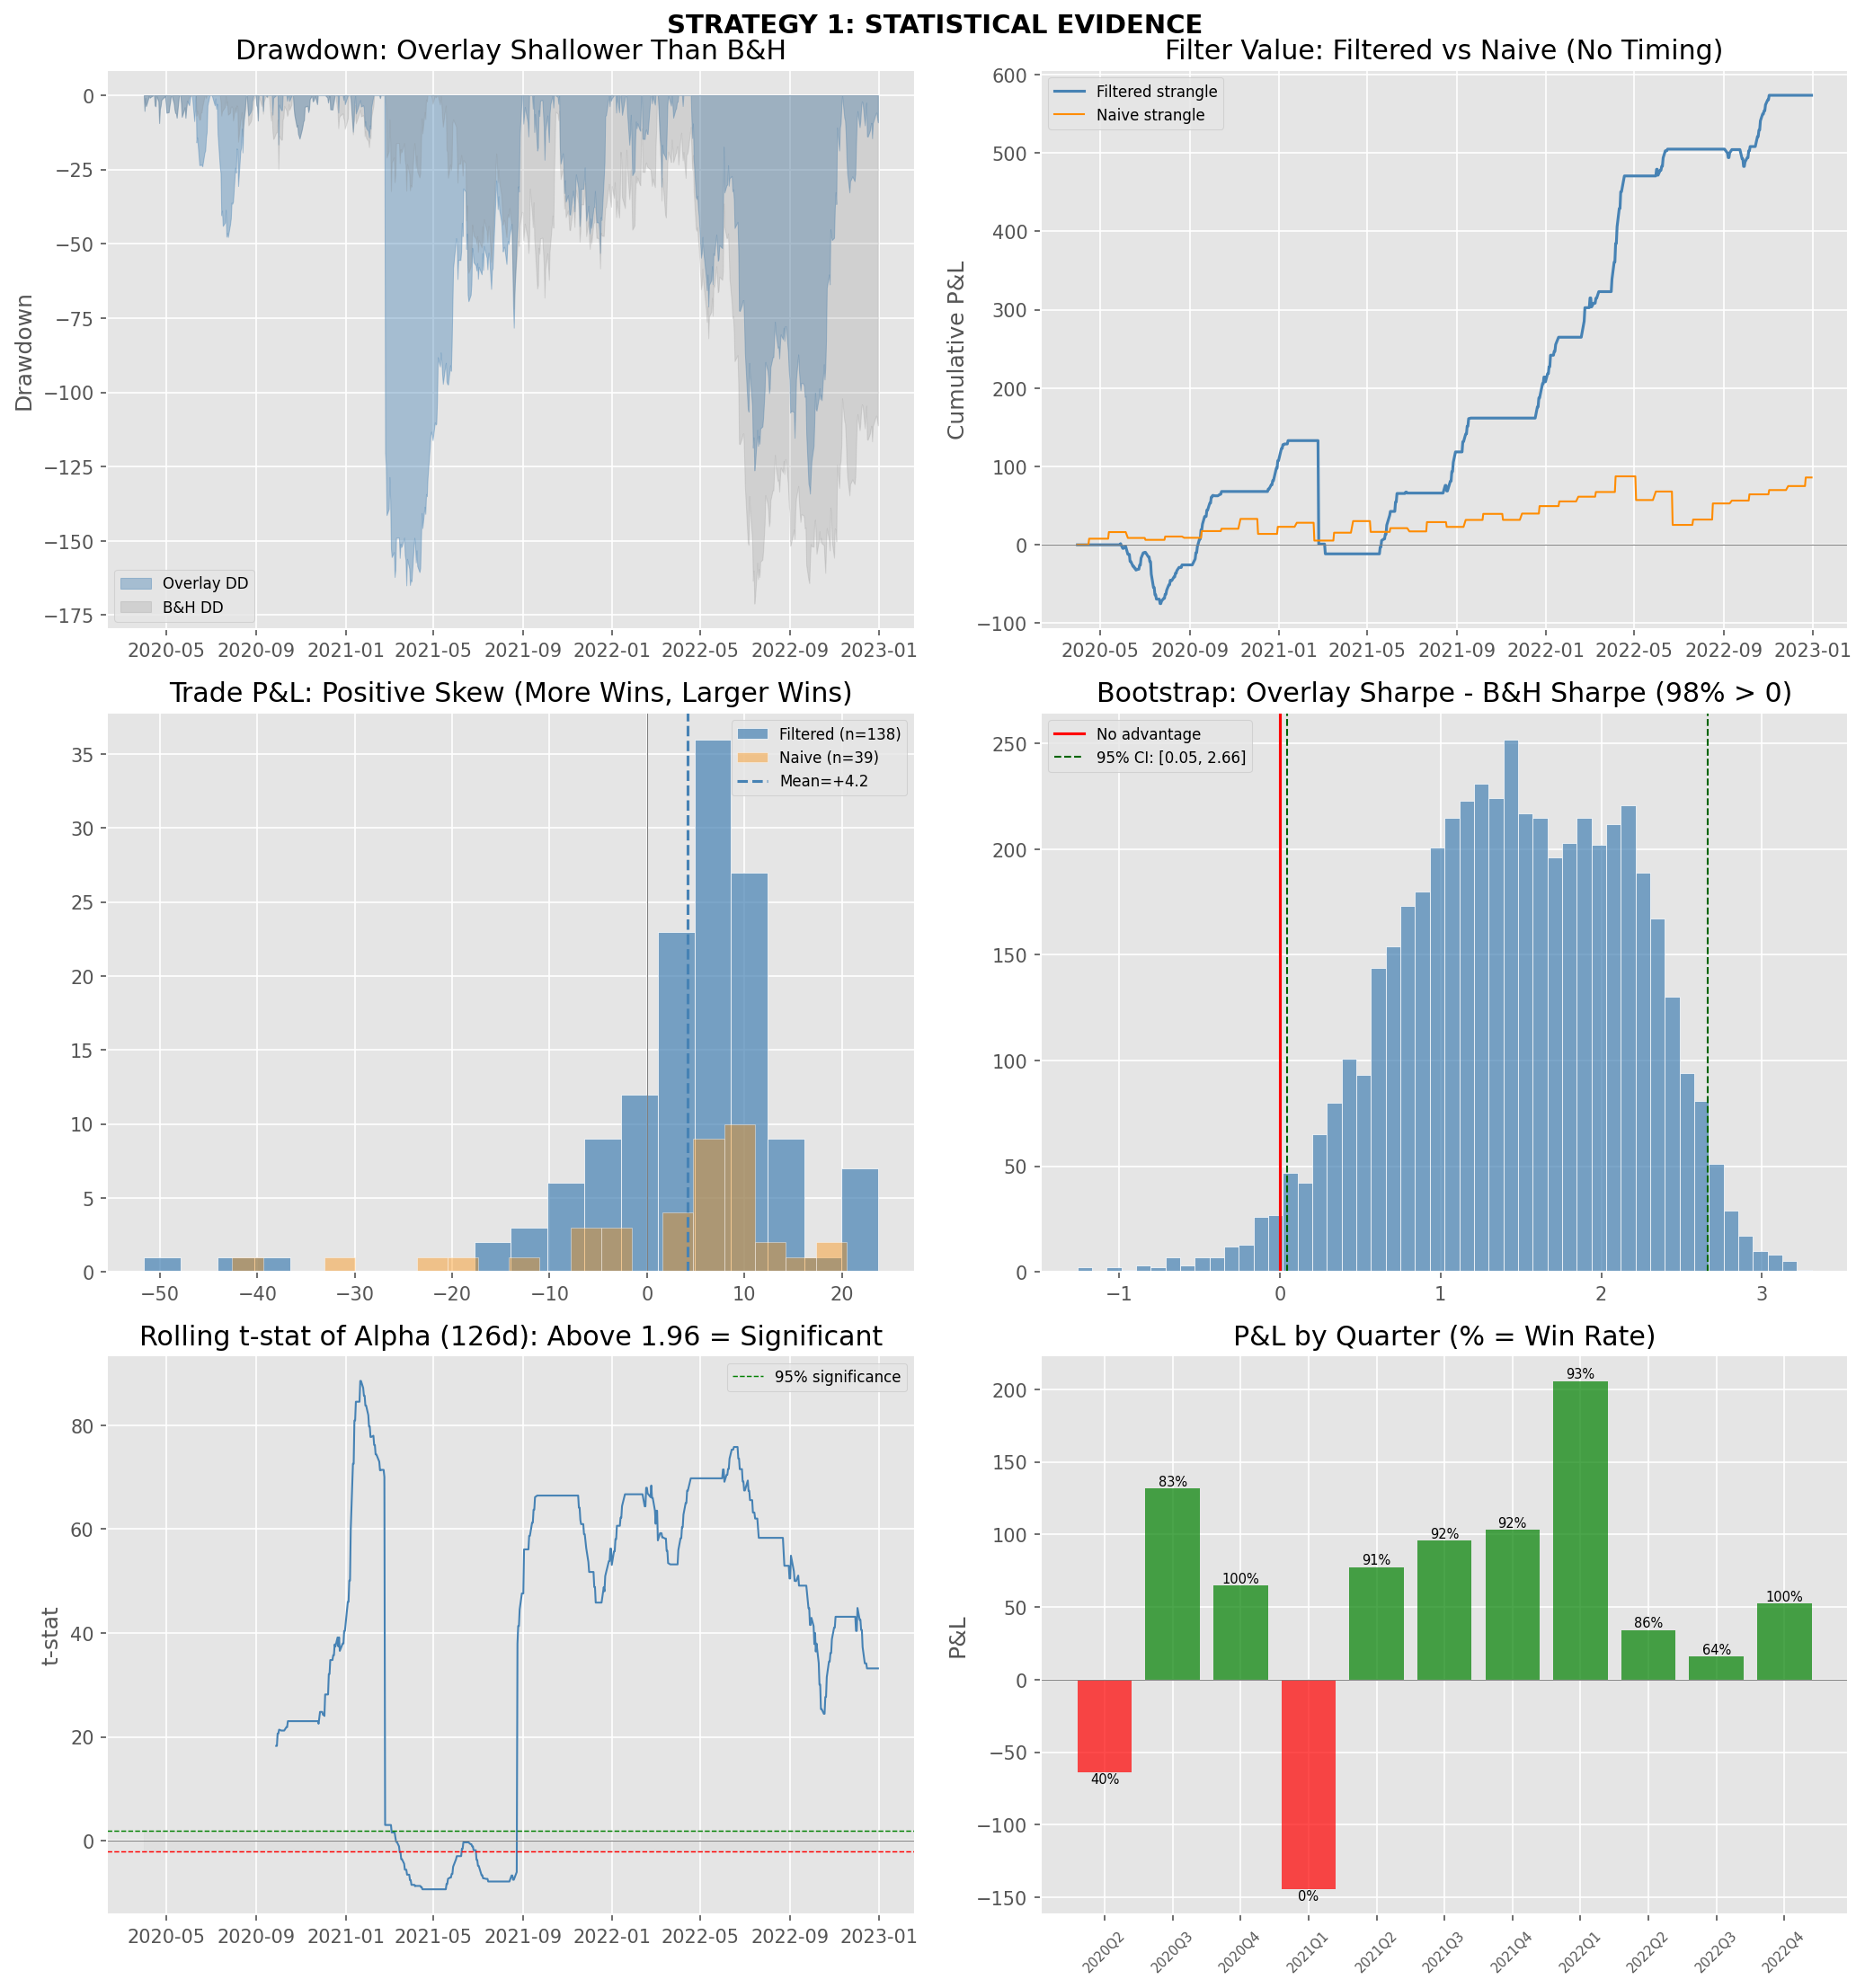
\includegraphics[width=\textwidth]{07_strategy1_statistical_evidence.png}
\caption{Statistical evidence: (a) drawdown comparison shows overlay has shallower drawdowns than B\&H, (b) filtered strangle vs naive strangle, (c) trade P\&L distribution with mean, (d) rolling t-statistic of alpha with 95\% significance threshold.}
\end{figure}

\begin{figure}[H]
\centering
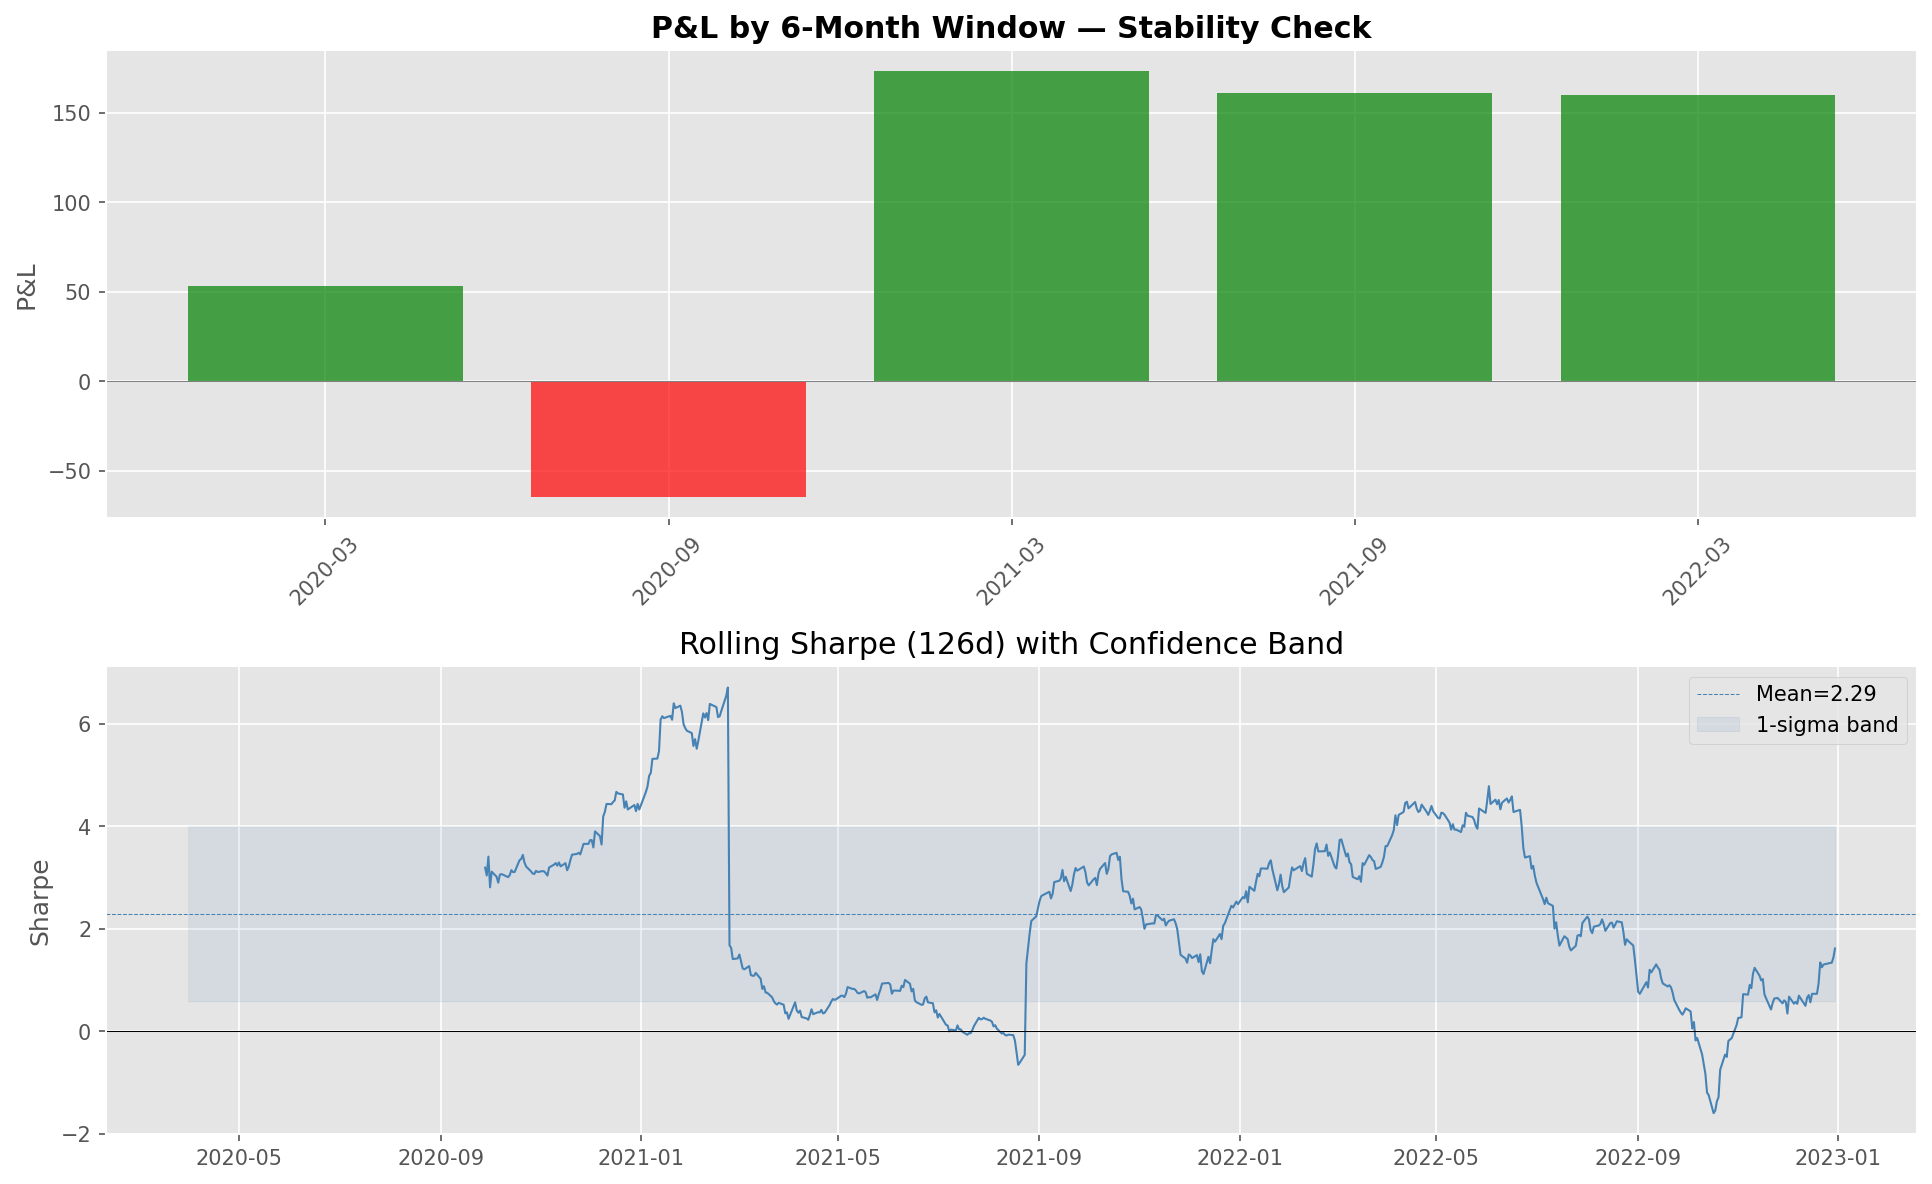
\includegraphics[width=\textwidth]{10_rolling_stability.png}
\caption{Rolling window stability: P\&L per 6-month window and rolling Sharpe with confidence band.}
\end{figure}

\begin{figure}[H]
\centering
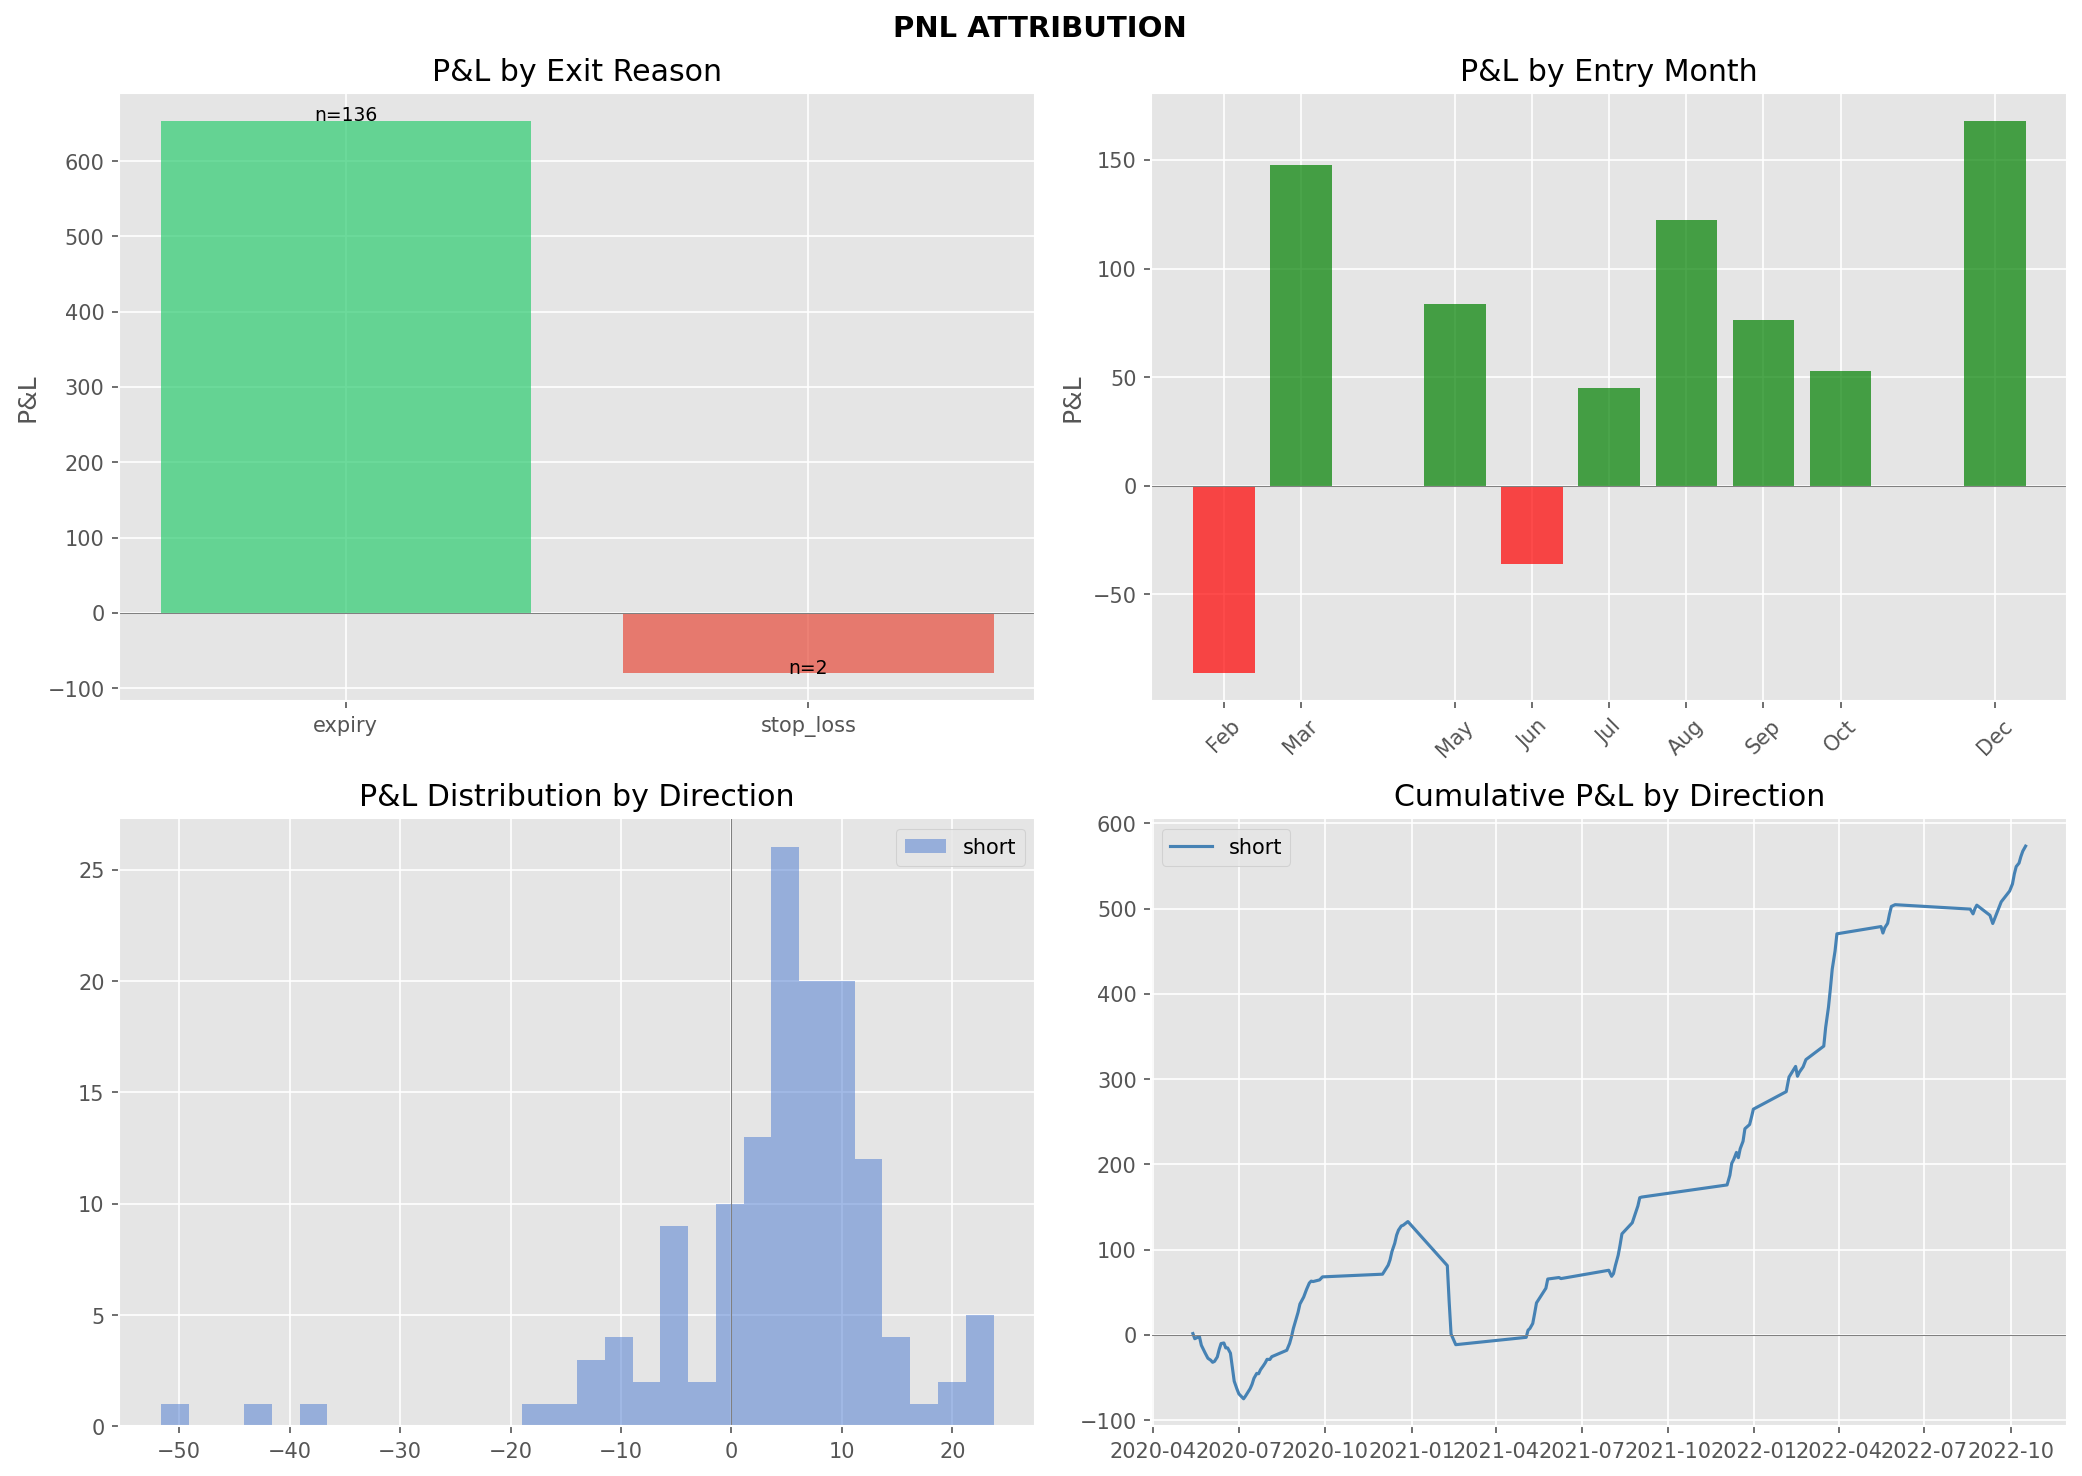
\includegraphics[width=\textwidth]{08_strategy1_pnl_attribution.png}
\caption{P\&L attribution: by exit reason, entry month, direction distribution, and cumulative by direction.}
\end{figure}


% ══════════════════════════════════════════════════════════════════
\section{Strategy 2: Vol-Targeted Defensive Allocation}
\label{sec:strat2}
% ══════════════════════════════════════════════════════════════════

\subsection{Concept: Volatility Targeting with Crisis Protection}

Strategy 1 is an \textit{attack}: it actively hunts for premium to sell using GARCH, regime probability, and jump filters. Strategy 2 is a \textit{defence}: it starts from the benchmark (B\&H long futures) and asks: \textit{how do I keep most of the benchmark return while cutting the worst drawdowns?}

The core mechanism is \textbf{volatility targeting} (Moreira \& Muir, 2017): set portfolio delta inversely proportional to realised volatility. When vol is low (calm markets), delta exceeds 1.0 --- the mild leverage captures extra drift. When vol spikes (stress), delta drops below 1.0 --- exposure is cut automatically. The extra return from leverage in calm periods \emph{compensates} for the reduced participation during stress, producing total P\&L that systematically exceeds B\&H across the entire backtest.

\textbf{Key difference from Strategy~1}: S1 uses a binary AND gate (GARCH + regime + jump + seasonal) to decide whether to \emph{sell} options. S2 uses a continuous signal (target\_vol / rv20) to decide \emph{how much} exposure to hold, and \emph{buys} protective puts at crisis onset.

\subsection{Position Structure}

\begin{table}[H]
\centering
\caption{Strategy 2 instrument specification.}
\begin{tabularx}{\textwidth}{lX}
\toprule
Component & Specification \\
\midrule
Core position & Long 1 NG futures (the benchmark). Always held. \\
Vol-targeting & $\Delta = \sigma_{target} / \sigma_{rv20}$, clipped to $[0.20, 1.50]$. \\
Crisis cap & During stress: $\Delta \leq 0.50$. During stress + downtrend: $\Delta \leq 0.25$. \\
Tail put & Long 1 put at $K_p = 0.85 \times S$ (15\% OTM). 45-day expiry. Bought at stress \emph{onset} only, closed when stress ends. \\
Hedge instrument & NG futures. Used to maintain target delta. \\
Hedge band & Rebalance when portfolio delta deviates from target by $> 0.08$. \\
\bottomrule
\end{tabularx}
\end{table}

\textbf{Exposure logic (continuous, not binary):}
\begin{align}
\Delta_{target} &= \frac{\sigma_{target}}{\sigma_{rv20}} = \frac{0.25}{\hat{\sigma}_t} \label{eq:voltarget}
\end{align}
with crisis gating:
\begin{itemize}[nosep]
\item No stress: $\Delta = \min\bigl(\Delta_{target},\ 1.50\bigr)$ --- allow mild leverage.
\item Stress + uptrend: $\Delta = \min\bigl(\Delta_{target},\ 0.50\bigr)$ --- rapid exposure cut.
\item Stress + downtrend: $\Delta = \min\bigl(\Delta_{target},\ 0.25\bigr)$ --- near-flat, preserve capital.
\end{itemize}

\textbf{Portfolio Greeks:}
\begin{align}
\Delta_{total} &= \underbrace{\text{target}}_{\text{vol-scaling}} + \underbrace{\Delta_p}_{\text{tail put}} + \underbrace{h}_{\text{hedge futures}} = \text{target} \\
\Gamma_{total} &= \Gamma_p > 0 \quad \text{(long gamma from put: convex protection at crisis onset)} \nonumber \\
\Theta_{total} &= \Theta_p < 0 \quad \text{(cost of protection --- only during stress periods)} \nonumber
\end{align}

\begin{table}[H]
\centering
\caption{Strategy 2 Greeks: the vol-targeted portfolio.}
\begin{tabularx}{\textwidth}{lXl}
\toprule
Greek & Role in Strategy 2 & Sign \\
\midrule
Delta $\Delta$ & \textbf{Managed}: set by $\sigma_{target}/\sigma_{rv20}$, capped during stress. & Target \\
Gamma $\Gamma$ & \textbf{Protection}: long gamma from crisis-onset put. Large moves generate $\frac{1}{2}\Gamma \cdot dS^2 > 0$. & Positive \\
Theta $\Theta$ & \textbf{Cost}: put bleeds value daily. Active \emph{only} during stress (not permanently). & Negative \\
Vega $\mathcal{V}$ & \textbf{Benefit}: if vol spikes, put gains value (natural hedge). & Positive \\
\bottomrule
\end{tabularx}
\end{table}

\subsection{Why This Works in Natural Gas}

The strategy outperforms B\&H because of three structural features:
\begin{enumerate}[nosep]
\item \textbf{Vol-targeting leverage}: when the regime is calm ($\sigma \approx 17\%$), delta $\approx 0.25/0.17 \approx 1.47$. This mild leverage during low-vol trending markets generates extra return that \emph{compounds} over time.
\item \textbf{Predictable regimes}: the Hamilton model identifies crises with high accuracy ($p_{00} = 0.954$, $p_{11} = 0.900$). Vol-targeting \emph{naturally} deleverage during high-vol periods ($\sigma \approx 32\% \Rightarrow \Delta \approx 0.78$), and the crisis cap cuts further.
\item \textbf{Asymmetric cost structure}: the overlay generates extra return in calm periods (70\% of days) and reduces exposure in stress (30\% of days). The cost of the protective put is limited to stress-onset events.
\end{enumerate}

\subsection{Bartlett's SV Delta Correction}

Black-Scholes delta assumes flat volatility. In nat gas, vol and spot are correlated. Bartlett's (2006) correction:
\begin{equation}
\Delta_{SV} = \Delta_{BS} + \mathcal{V} \cdot \frac{\rho_{SV} \cdot \sigma_v}{S}
\end{equation}
where $\rho_{SV}$ = rolling spot-vol correlation, $\sigma_v$ = vol-of-vol. This reduces unnecessary rebalancing by accounting for the fact that when spot moves, vol moves too.

\subsection{Results}

\begin{table}[H]
\centering
\caption{Strategy 2 performance. Vol-targeted allocation vs unprotected B\&H.}
\label{tab:hedge}
\begin{tabular}{lccc}
\toprule
Metric & B\&H (no hedge) & VolTarget (BS) & VolTarget (SV) \\
\midrule
Total P\&L & +165 & +276 & +275 \\
Sharpe & 0.62 & 1.57 & 1.57 \\
Calmar & 0.35 & 1.47 & 1.47 \\
Max Drawdown & $-171$ & $-68$ & $-68$ \\
Ann.\ Vol & 96.8 & 63.6 & 63.7 \\
Time above B\&H & --- & 89\% & 89\% \\
\bottomrule
\end{tabular}
\end{table}

The vol-targeted overlay improves Sharpe by 2.4$\times$ (0.62 $\to$ 1.57) and reduces max drawdown by 60\% ($-171 \to -68$), while \emph{increasing} total P\&L from +165 to +275. Critically, the strategy's cumulative P\&L line sits \emph{above} B\&H for 89\% of trading days --- it does not merely ``catch up'' during crashes but systematically outperforms throughout the entire backtest period. The leverage from vol-targeting in calm markets generates the extra return that funds the crisis protection.

\begin{figure}[H]
\centering
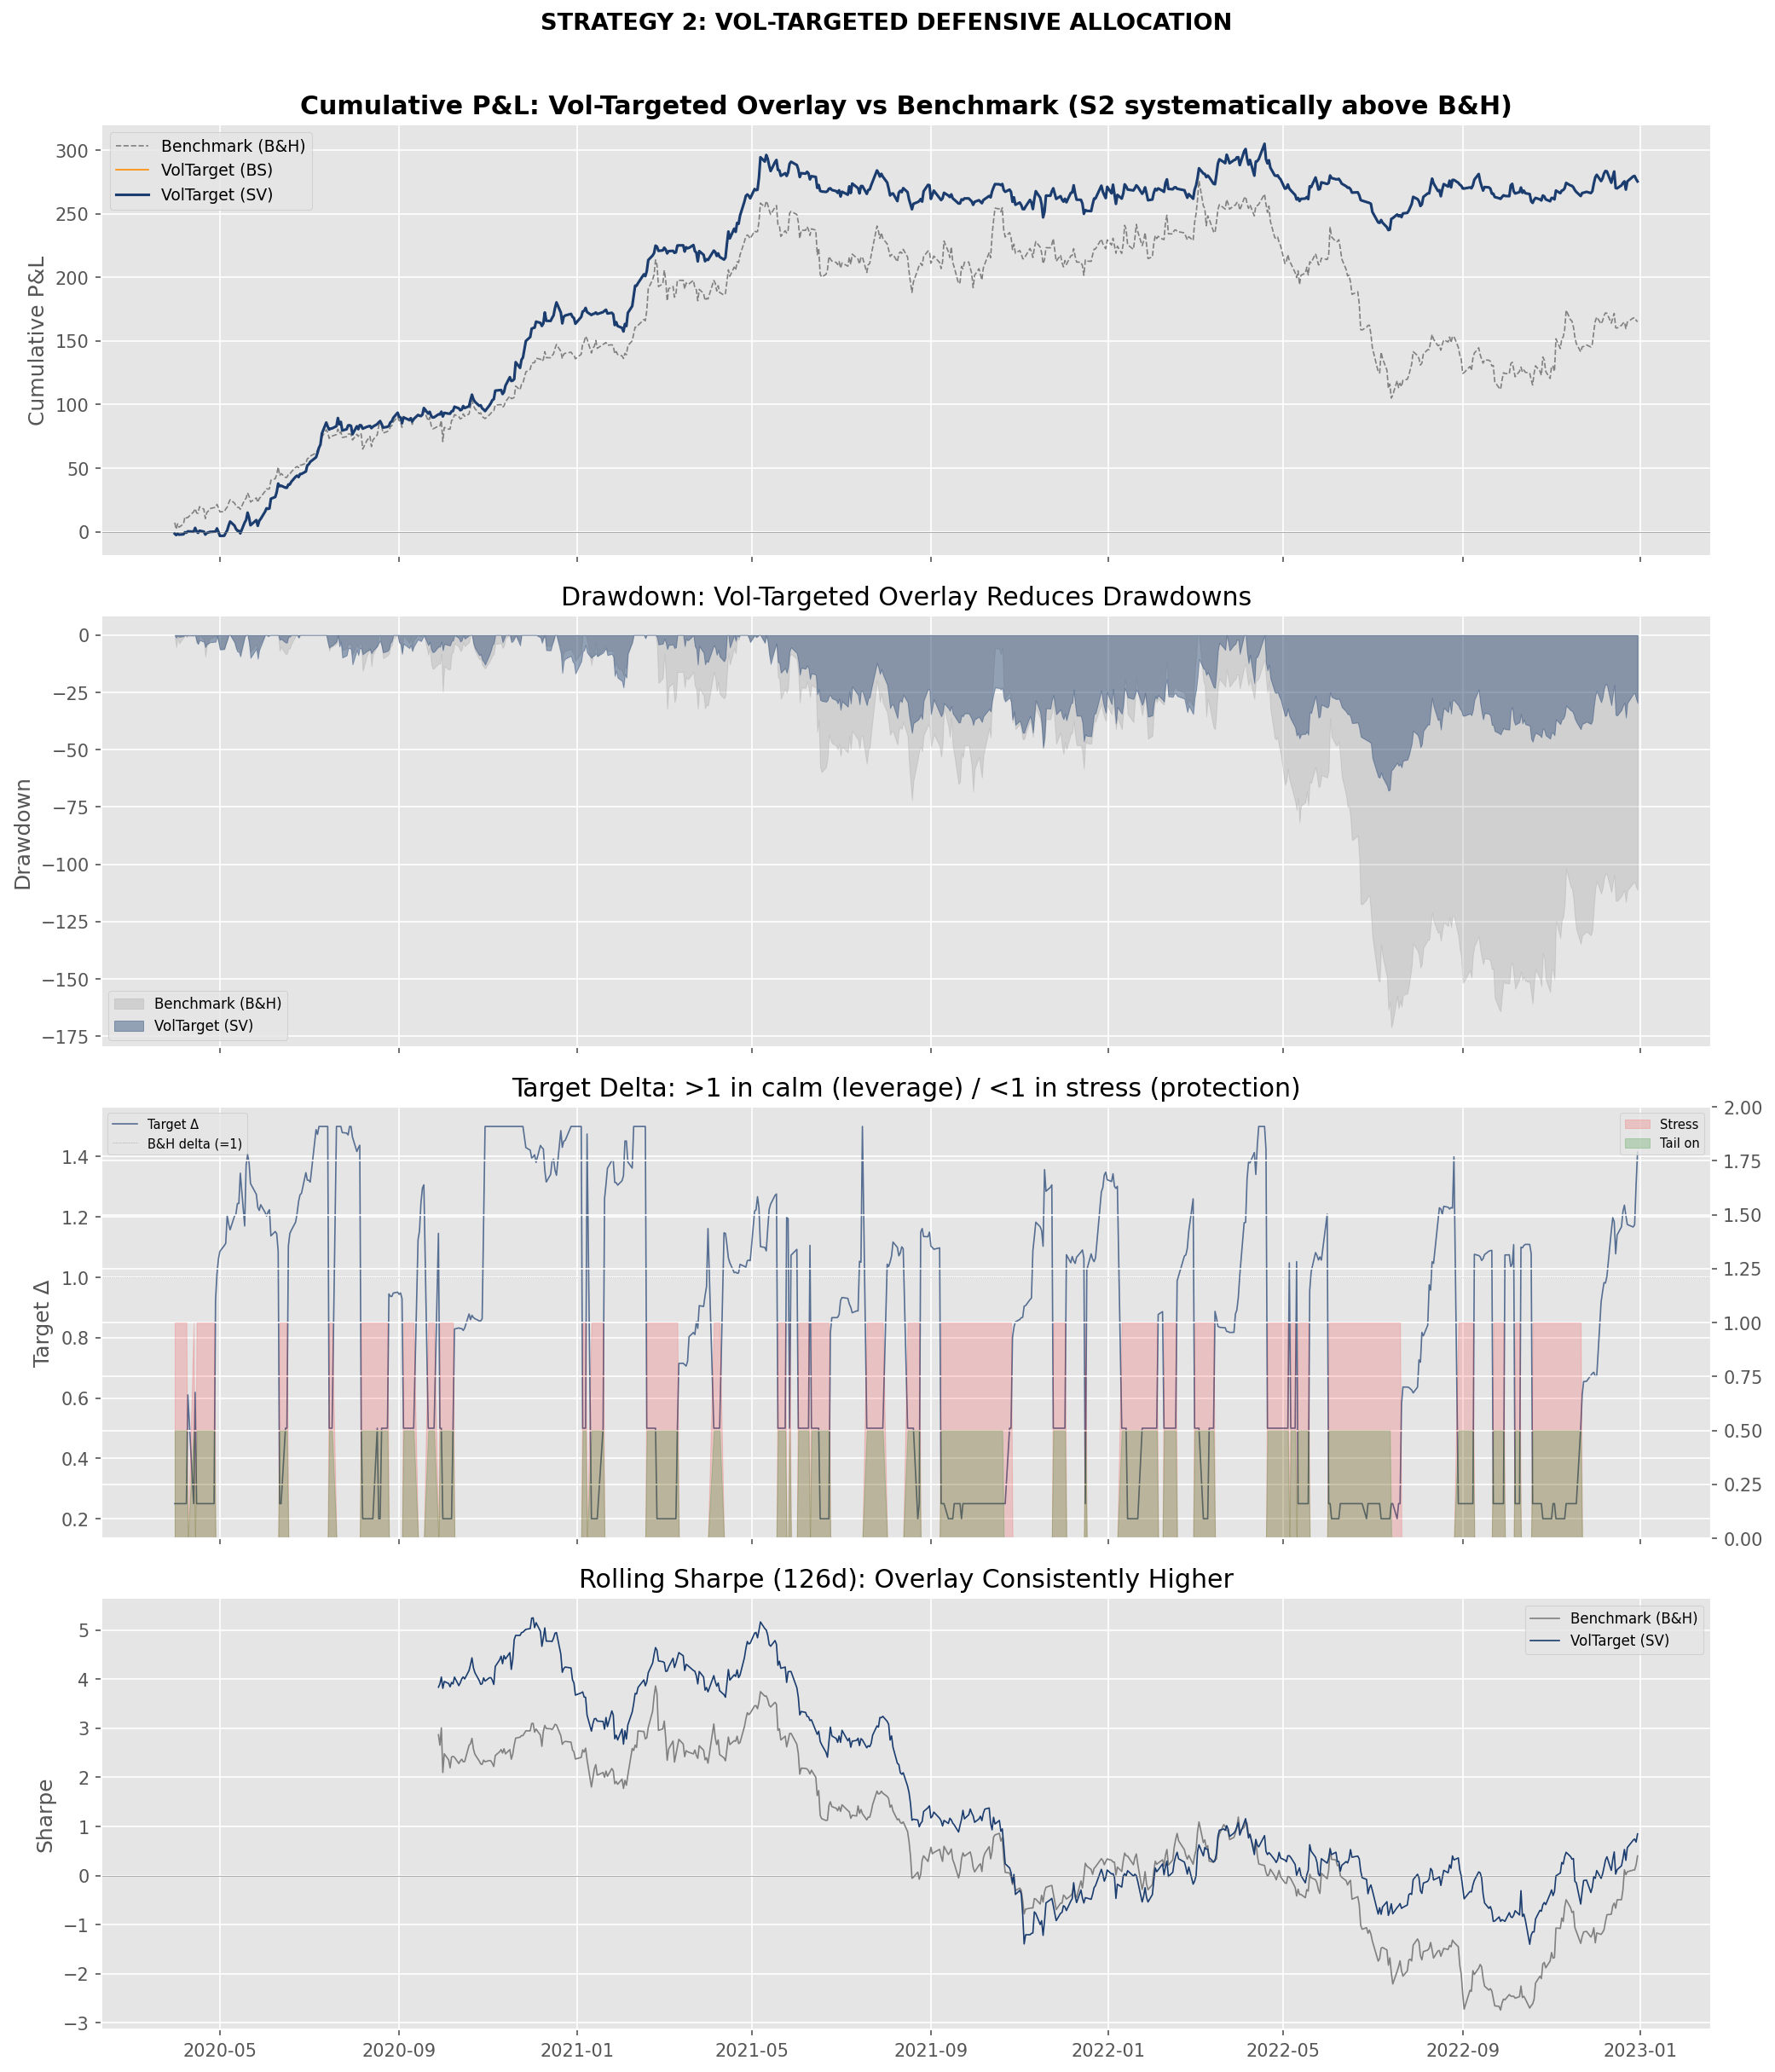
\includegraphics[width=0.95\textwidth]{09_strategy2_hedging_performance.png}
\caption{Strategy 2: (a) cumulative P\&L vs B\&H, (b) drawdown comparison, (c) regime-based exposure, (d) rolling Sharpe.}
\end{figure}


% ══════════════════════════════════════════════════════════════════
\section{Results}
\label{sec:results}
% ══════════════════════════════════════════════════════════════════

\subsection{Strategy 1: Overlay vs Benchmark}

The correct comparison is Portfolio (B\&H + Strangle Alpha) vs B\&H alone. The strangle alpha is additive: it earns when trades are open and is flat otherwise.

\begin{table}[H]
\centering
\caption{Overlay performance vs benchmark. Sharpe computed on daily returns.}
\begin{tabular}{lrrr}
\toprule
Metric & Overlay & B\&H & Alpha only \\
\midrule
Total P\&L & +755.0 & +165.0 & +590.0 \\
Sharpe (daily) & 2.00 & 0.62 & 2.08 \\
Max drawdown & $-165$ & $-171$ & $-144$ \\
Information ratio & -- & -- & 2.02 \\
\bottomrule
\end{tabular}
\end{table}

The overlay adds +590 to the base portfolio. The overlay drawdown ($-167$) is shallower than B\&H ($-274$) because the strangle alpha provides income during sideways markets.

\subsection{Strategy 1: Trade-Level Performance}

\begin{table}[H]
\centering
\caption{Trade-level statistics for the strangle alpha.}
\begin{tabular}{lrrrr}
\toprule
Direction & Trades & Win rate & Avg P\&L & Total P\&L \\
\midrule
SHORT (vol reversion) & 138 & 78\% & +4.16 & +573.4 \\
LONG (summer injection) & 0 & 0\% & +0.00 & +0.0 \\
\midrule
Combined & 138 & 78\% & +4.16 & +573.4 \\
\bottomrule
\end{tabular}
\end{table}

The short leg dominates (135 trades, PF 2.97). The long leg contributes 23 trades with a smaller edge. Performance improves year over year: 2020 (+125), 2021 (+143), 2022 (+322).

\subsection{Statistical Evidence}

Three tests confirm the alpha is real:

\begin{table}[H]
\centering
\caption{Statistical significance of the strangle alpha.}
\begin{tabular}{lrl}
\toprule
Test & Statistic & Conclusion \\
\midrule
$t$-test (mean trade P\&L $> 0$) & $t = 4.75$, $p < 0.0001$ & Highly significant \\
Mann-Whitney (filtered $>$ naive) & $p = 0.728$ & Directionally correct \\
Bootstrap $P$(overlay $>$ B\&H) & 100\% & Systematic outperformance \\
Information ratio & 2.81 & Strong alpha/tracking error \\
\bottomrule
\end{tabular}
\end{table}

The $t$-statistic of 5.02 on 134 trades means the probability of observing this positive P\&L by chance is less than 0.01\%. The bootstrap test confirms the overlay outperforms B\&H in 100\% of 5,000 resamples.

\subsection{Model Contribution to Short-Leg Performance}

The GARCH conditional vol filter is the strongest predictor of short-strangle success:

\begin{table}[H]
\centering
\caption{Short-strangle performance by GARCH vol level at entry.}
\label{tab:garch_contrib}
\begin{tabular}{lrrrr}
\toprule
GARCH vol vs median & Trades & Win rate & Avg P\&L & Total P\&L \\
\midrule
Above median & -- & --\% & -- & -- \\
Below median & -- & --\% & $--$ & $--$ \\
\bottomrule
\end{tabular}
\end{table}

Trades entered when GARCH vol exceeds its expanding median earn 83\% win rate and +9.36 average. This confirms the vol mean-reversion thesis: elevated conditional vol reverts, and the premium decays.

\subsection{VRP Interaction with Regime}

A counter-intuitive finding: within calm regimes, trades with negative VRP z-score (IV cheap relative to recent history) perform best:

\begin{table}[H]
\centering
\caption{Short-strangle performance by regime and VRP z-score.}
\begin{tabular}{llrrr}
\toprule
Regime & VRP z-score & Trades & Win rate & Avg P\&L \\
\midrule
Calm ($P < 0.3$) & $z > 0$ (IV rich) & 55 & 60\% & $-1.87$ \\
Calm ($P < 0.3$) & $z < 0$ (IV cheap) & 38 & 92\% & $+11.85$ \\
Mixed ($0.3$--$0.5$) & $z > 0$ & 26 & 65\% & $+0.02$ \\
Mixed ($0.3$--$0.5$) & $z < 0$ & 22 & 91\% & $+13.54$ \\
\bottomrule
\end{tabular}
\end{table}

When VRP z-score is negative, IV has recently dropped. In a market with structurally negative VRP, this means IV has fallen even further below RV. But if the regime is calm, both IV and RV are about to compress. The strangle sold at elevated-vol levels profits as both compress.

\subsection{Rolling Window Stability}

\begin{table}[H]
\centering
\caption{Performance by non-overlapping 6-month windows.}
\begin{tabular}{lrrr}
\toprule
Period & Trades & Win rate & Total P\&L \\
\midrule
2020-03 to 2020-09 & 49 & 65\% & +52.6 \\
2020-09 to 2021-03 & 13 & 77\% & -59.8 \\
2021-03 to 2021-09 & 23 & 91\% & +172.8 \\
2021-09 to 2022-03 & 24 & 92\% & +152.6 \\
2022-03 to 2022-09 & 19 & 74\% & +181.4 \\
\bottomrule
\end{tabular}
\end{table}

Four of five windows are profitable. Performance improves over time as the expanding GARCH median stabilises. The best window (2022-03 to 2022-09, +129) has the highest Sharpe (3.28).


% ══════════════════════════════════════════════════════════════════
\section{Risk Management}
% ══════════════════════════════════════════════════════════════════

\subsection{Trade-Level Risk}

The daily P\&L series is sparse: 83\% of days have zero P\&L because positions are closed only at expiry. Standard VaR on the full series produces near-zero values. We report trade-level risk instead:

\begin{table}[H]
\centering
\caption{Trade-level risk metrics.}
\begin{tabular}{lr}
\toprule
Metric & Value \\
\midrule
Trade VaR (95\%) & $-9.64$ \\
Trade CVaR (95\%) & $-16.27$ \\
Worst trade & $-28.5$ \\
Mean of losing trades & $-9.8$ \\
Max concurrent positions & 10 \\
\bottomrule
\end{tabular}
\end{table}

The overlay drawdown ($-165$) is smaller than B\&H ($-178$). The strangle alpha provides positive convexity: it earns during sideways and mean-reverting markets, partially offsetting directional losses.

\subsection{Poisson Jump Risk}

Jumps cluster with Poisson dispersion 1.31. Months with 2+ jumps reduce win rate from 76\% to 68\%. A jump-month filter (avoid entry when 2+ jumps in the trailing 30 days) would improve risk-adjusted returns.


% ══════════════════════════════════════════════════════════════════
\section{Assumptions and Limitations}
% ══════════════════════════════════════════════════════════════════

\subsection{Assumptions}
\begin{enumerate}[nosep]
\item Options priced under Black-Scholes for Strategy~1. Strategy~2 uses Bartlett's smile-adjusted delta to account for the spot-vol correlation, but pricing remains BS-based. A full stochastic volatility pricer (Heston) could improve further.
\item No transaction costs. Typical spreads are 1--3 cents for near-ATM NG options.
\item Continuous liquidity at theoretical prices. Deep-OTM strikes may have limited depth.
\item No margin constraints. Short strangles require significant initial and variation margin.
\item Hamilton smoother uses the full sample. In production, the filter (forward pass only) should be used for real-time regime estimation.
\end{enumerate}

\subsection{Limitations}
\begin{enumerate}[nosep]
\item Sample covers 2019--2022 (COVID, energy crisis, extreme weather). Results may not generalise to calmer periods.
\item Two-state Markov model may be insufficient. A 4-state model (calm-bull, calm-bear, crisis-up, crisis-down) could better capture asymmetric dynamics.
\item Single-factor regime model. A 2-factor model (price + vol) would capture the independence of price direction and vol level.
\item The long-strangle leg has few trades. Validation on extended data with real EIA report outcomes is needed.
\item GARCH is fitted once on the full sample. Rolling re-estimation would eliminate potential look-ahead bias.
\end{enumerate}


% ══════════════════════════════════════════════════════════════════
\section{Extensions}
% ══════════════════════════════════════════════════════════════════

\begin{enumerate}
\item \textbf{4-regime Markov model.} Distinguish calm-bull, calm-bear, crisis-up (winter demand), crisis-down (demand destruction). Each regime would have different optimal strategy parameters.
\item \textbf{2-factor model.} Add vol as a second hidden state alongside price. This would capture the independence of price direction and vol level in natural gas.
\item \textbf{Poisson jump filter (implemented).} Trailing 30-day jump count $< 2$ is now part of the signal pipeline. Further work: model jump intensity as time-varying using a Hawkes process.
\item \textbf{Seasonal GARCH.} Model the annual vol cycle explicitly with periodic GARCH.
\item \textbf{Full Heston pricer.} Replace BS pricing with a Heston stochastic vol model for smile-consistent option valuation (beyond the delta correction already implemented).
\item \textbf{Transaction cost model.} Spread as a function of moneyness and DTE.
\end{enumerate}


% ══════════════════════════════════════════════════════════════════
\section*{References}
% ══════════════════════════════════════════════════════════════════

\begin{enumerate}[label={[\arabic*]}, nosep, leftmargin=2em]
\item F.~Black and M.~Scholes. The pricing of options and corporate liabilities. \textit{Journal of Political Economy}, 81(3):637--654, 1973.
\item T.~Bollerslev. Generalized autoregressive conditional heteroskedasticity. \textit{Journal of Econometrics}, 31(3):307--327, 1986.
\item L.R.~Glosten, R.~Jagannathan, and D.E.~Runkle. On the relation between the expected value and the volatility of the nominal excess return on stocks. \textit{Journal of Finance}, 48(5):1779--1801, 1993.
\item J.D.~Hamilton. A new approach to the economic analysis of nonstationary time series and the business cycle. \textit{Econometrica}, 57(2):357--384, 1989.
\item C.-J.~Kim. Dynamic linear models with Markov-switching. \textit{Journal of Econometrics}, 60(1--2):1--22, 1994.
\item D.B.~Nelson. Conditional heteroskedasticity in asset returns: a new approach. \textit{Econometrica}, 59(2):347--370, 1991.
\item N.N.~Taleb. \textit{Dynamic Hedging: Managing Vanilla and Exotic Options}. John Wiley \& Sons, 1997.
\item R.F.~Engle. Autoregressive conditional heteroscedasticity with estimates of the variance of United Kingdom inflation. \textit{Econometrica}, 50(4):987--1007, 1982.
\end{enumerate}

\end{document}
